%
% $RCSfile: paper.tex,v $
%
% Copyright (c) 2001-2004. Christian Heller. All rights reserved.
%
% No copying, altering, distribution or any other actions concerning this
% document, except after explicit permission by the author!
% At some later point in time, this document is planned to be put under
% the GNU FDL license. For now, _everything_ is _restricted_ by the author.
%
% http://www.cybop.net
% - Cybernetics Oriented Programming -
%
% http://www.resmedicinae.org
% - Information in Medicine -
%
% @author Christian Heller <christian.heller@tuxtax.de>
%

%
% The document class specifying the type of document.
%
\documentclass[a4paper,10pt]{llncs}

%
% The usepackages for document class.
%

% Paper format and font.
\usepackage{a4,times,helvet}

% Graphics.
\usepackage{graphicx}

%
% The space settings for edges (left, top, right, bottom).
%
\setlength{\hoffset}{-1,3in}
\setlength{\voffset}{-1in}
\setlength{\oddsidemargin}{3,5cm}
\setlength{\topmargin}{1,3cm}
%\setlength{\headwidth}{16,5cm}
\setlength{\headheight}{0cm}
\setlength{\textwidth}{16,5cm}
\setlength{\textheight}{23,2cm}

%
% The hyphenation list.
%
%
% $RCSfile: hyphenation.tex,v $
%
% Copyright (c) 2001-2004. Christian Heller. All rights reserved.
%
% No copying, altering, distribution or any other actions concerning this
% document, except after explicit permission by the author!
% At some later point in time, this document is planned to be put under
% the GNU FDL license. For now, _everything_ is _restricted_ by the author.
%
% http://www.cybop.net
% - Cybernetics Oriented Programming -
%
% http://www.resmedicinae.org
% - Information in Medicine -
%
% @author Christian Heller <christian.heller@tuxtax.de>
%

\hyphenation{abs-trac-tion}
\hyphenation{abs-trac-tions}
\hyphenation{ac-tu-ally}
\hyphenation{addi-tio-nally}
\hyphenation{ana-lyst}
\hyphenation{ana-ly-sis}
\hyphenation{an-cient}
\hyphenation{ap-pli-ca-tion}
\hyphenation{arche-types}
\hyphenation{aris-to-tle}
\hyphenation{at-tri-bute}
\hyphenation{avoi-da-ble}
\hyphenation{be-ing}
\hyphenation{binary}
\hyphenation{bran-ches}
\hyphenation{ca-te-go-ri-za-tion}
\hyphenation{client}
\hyphenation{com-po-nen-ti-za-tion}
\hyphenation{com-pu-ter}
\hyphenation{con-fi-gure}
\hyphenation{con-fi-gu-ra-tion}
\hyphenation{con-nec-ted}
\hyphenation{cri-ti-cised}
\hyphenation{cy-ber-ne-tics}
\hyphenation{cyboi}
\hyphenation{cybol}
\hyphenation{cybop}
\hyphenation{de-sign}
\hyphenation{des-cribe}
\hyphenation{des-cribed}
\hyphenation{de-ve-lop-ment}
\hyphenation{dis-crete}
\hyphenation{di-vide}
\hyphenation{do-main}
\hyphenation{dy-na-mic}
\hyphenation{dy-na-mics}
\hyphenation{ela-bo-ra-ted}
\hyphenation{ele-ments}
\hyphenation{en-gi-nee-ring}
\hyphenation{eng-lish}
\hyphenation{en-vi-ron-ment}
\hyphenation{ex-pert}
\hyphenation{fi-gure}
\hyphenation{fun-da-men-tal}
\hyphenation{func-tio-na-li-ty}
\hyphenation{hard-ware}
\hyphenation{hu-man}
\hyphenation{im-ple-men-ta-tion}
\hyphenation{imp-roved}
\hyphenation{in-he-rit}
\hyphenation{in-ter-pre-ter}
\hyphenation{java}
\hyphenation{know-ledge}
\hyphenation{lan-guage}
\hyphenation{li-ving}
\hyphenation{lo-gi-cal}
\hyphenation{machine}
\hyphenation{me-cha-nism}
\hyphenation{me-thods}
\hyphenation{na-ture}
\hyphenation{net-work}
\hyphenation{neu-ral}
\hyphenation{neu-ron}
\hyphenation{nu-me-rous}
\hyphenation{object}
\hyphenation{open}
\hyphenation{operating}
\hyphenation{ori-en-ted}
\hyphenation{over-come}
\hyphenation{prin-ci-ple}
\hyphenation{prin-ting}
\hyphenation{pro-ba-bi-lis-tic}
\hyphenation{pro-gram-ming}
\hyphenation{re-cog-nize}
\hyphenation{re-cog-nized}
\hyphenation{re-pre-sen-ta-tion}
\hyphenation{re-pre-sen-ting}
\hyphenation{re-u-sa-bi-li-ty}
\hyphenation{sci-ence}
\hyphenation{server}
\hyphenation{se-pa-ra-ted}
\hyphenation{se-pa-ra-tion}
\hyphenation{si-mi-lar}
\hyphenation{soft-ware}
\hyphenation{source}
\hyphenation{spe-cia-li-za-tion}
\hyphenation{sta-tic}
\hyphenation{sta-ti-cal-ly}
\hyphenation{sto-chas-tic}
\hyphenation{stone-on-stone}
\hyphenation{struc-ture}
\hyphenation{strug-gling}
\hyphenation{su-per-flu-ous}
\hyphenation{sup-ply-ing}
\hyphenation{sys-tem}
\hyphenation{tes-ting}
\hyphenation{thin-king}
\hyphenation{un-en-li-vened}
\hyphenation{un-fa-vou-ra-ble}
\hyphenation{un-sa-tis-fy-ing}
\hyphenation{va-ry-ing}
\hyphenation{weigh-ted}


%
% This document is a scientific paper to be handed in for a conference.
%
% @version $Revision: 1.1 $ $Date: 2003-10-08 12:40:03 $ $Author: christian $
% @author Christian Heller <christian.heller@tuxtax.de>
% @author Christian Heller <christian.heller@tu-ilmenau.de>
%
\begin{document}
    \twocolumn
    %
% $RCSfile: title.tex,v $
%
% Copyright (c) 2001-2004. Christian Heller. All rights reserved.
%
% No copying, altering, distribution or any other actions concerning this
% document, except after explicit permission by the author!
% At some later point in time, this document is planned to be put under
% the GNU FDL license. For now, _everything_ is _restricted_ by the author.
%
% http://www.cybop.net
% - Cybernetics Oriented Programming -
%
% http://www.resmedicinae.org
% - Information in Medicine -
%
% @author Christian Heller <christian.heller@tuxtax.de>
%

\title{A new Pattern Systematics}
\author{
    Christian Heller \(<\)christian.heller@tu-ilmenau.de\(>\)\\
    Detlef Streitferdt \(<\)detlef.streitferdt@tu-ilmenau.de\(>\)\\
    Ilka Philippow \(<\)ilka.philippow@tu-ilmenau.de\(>\)
}
\institute{Technical University of Ilmenau\\
    Faculty for Computer Science and Automation\\
    Institute for Theoretical and Technical Informatics\\
    PF 100565, Max-Planck-Ring 14, 98693 Ilmenau, Germany\\
    http://www.tu-ilmenau.de, fon: +49-3677-69-1230, fax: +49-3677-69-1220 \vspace*{0.5cm}
}

    \maketitle
    %
% $RCSfile: abstract.tex,v $
%
% Copyright (c) 2001-2004. Christian Heller. All rights reserved.
%
% No copying, altering, distribution or any other actions concerning this
% document, except after explicit permission by the author!
% At some later point in time, this document is planned to be put under
% the GNU FDL license. For now, _everything_ is _restricted_ by the author.
%
% http://www.cybop.net
% - Cybernetics Oriented Programming -
%
% http://www.resmedicinae.org
% - Information in Medicine -
%
% @author Christian Heller <christian.heller@tuxtax.de>
%

\begin{center}
    \textbf{\large{Abstract}}
\end{center}
\normalsize
\textit{
This document describes how existing design patterns can be combined to merge
their advantages into one domain- independent software framework. This framework,
called Cybernetics Oriented Programming (CYBOP), is characterized by flexibility
and extensibility. Further, the concept of Ontology is used to structure the
software architecture as well as to keep it maintainable. A Component Lifecycle
ensures the proper startup and shutdown of any systems built on top of CYBOP.\\
The practical proof of these new concepts was accomplished within the diploma
thesis of Jens Bohl which consisted of designing and developing a module called
Record, of the Open Source Software (OSS) project Res Medicinae. The major task
of this module is to provide a user interface for creating medical documentation.
New structure models such as Episodes were considered and implemented. In this
context, the integration of a graphical tool for Topological Documentation was
also highly demanded. The tool allows documentation with the help of anatomical
images and the setting of markers for pathological findings.\\
\textbf{Keywords.} Design Pattern, Framework, Component Lifecycle, Ontology,
CYBOP, Res Medicinae, Episode Based Documentation, Topological Documentation
} \rm


    %
% $RCSfile: introduction.tex,v $
%
% Copyright (c) 2005-2006. Christian Heller. All rights reserved.
%
% Permission is granted to copy, distribute and/or modify this document
% under the terms of the GNU Free Documentation License, Version 1.1 or
% any later version published by the Free Software Foundation; with no
% Invariant Sections, with no Front-Cover Texts and with no Back-Cover
% Texts. A copy of the license is included in the section entitled
% "GNU Free Documentation License".
%
% http://www.cybop.net
% - Cybernetics Oriented Programming -
%
% http://www.resmedicinae.org
% - Information in Medicine -
%
% Version: $Revision: 1.1 $ $Date: 2006-01-03 08:21:45 $ $Author: christian $
% Authors: Christian Heller <christian.heller@tuxtax.de>
%

\section{Introduction}
\label{introduction_heading}

Sometimes, describing the easy things is the most difficult. And most of the
time, it seems easier to copy existing concepts than to investigate new, but
possibly more intuitive solutions. The work described in this document tried to
question traditional concepts of software design and to correct or simplify
these by applying new ideas stemming from other scientific disciplines. It thus
wants to contribute to a better knowledge modelling.

The initially observed discrepancies belong to software engineering processes
(abstraction gaps), to the physical architecture (misleading tiers) as well as
the logical architecture (modelling mistakes) of systems. They are explained
following.

%
% $RCSfile: abstraction_gaps.tex,v $
%
% Copyright (c) 2005-2006. Christian Heller. All rights reserved.
%
% Permission is granted to copy, distribute and/or modify this document
% under the terms of the GNU Free Documentation License, Version 1.1 or
% any later version published by the Free Software Foundation; with no
% Invariant Sections, with no Front-Cover Texts and with no Back-Cover
% Texts. A copy of the license is included in the section entitled
% "GNU Free Documentation License".
%
% http://www.cybop.net
% - Cybernetics Oriented Programming -
%
% http://www.resmedicinae.org
% - Information in Medicine -
%
% Version: $Revision: 1.1 $ $Date: 2006-01-03 08:21:45 $ $Author: christian $
% Authors: Christian Heller <christian.heller@tuxtax.de>
%

\subsection{Abstraction Gaps}
\label{abstraction_gaps_heading}

Software has to be developed in a creative process called
\emph{Software Engineering Process} (SEP) or \emph{-Methodology} (figure
\ref{gaps_figure}).

\begin{figure}[htb]
    \begin{center}
        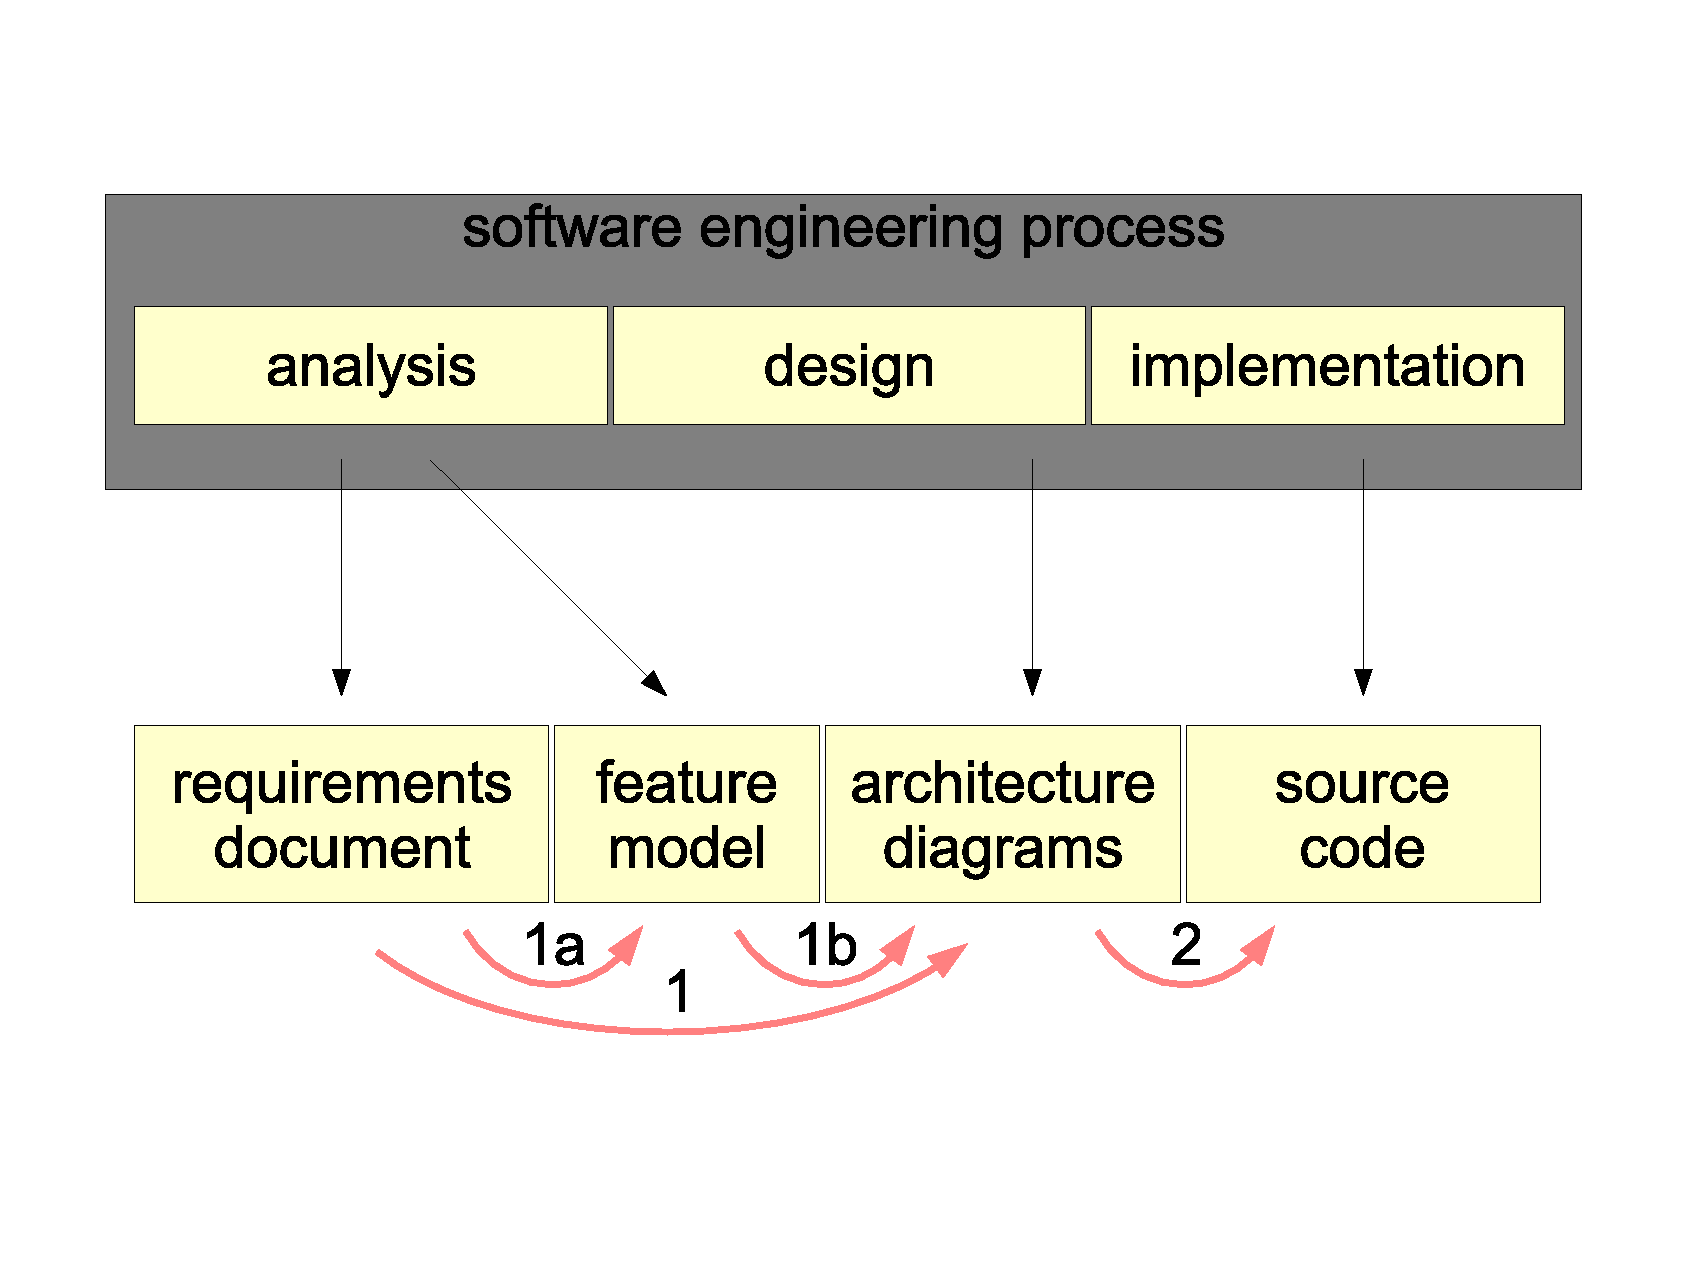
\includegraphics[scale=0.2]{vector/gaps.eps}
        \caption{Abstraction Gaps}
        \label{gaps_figure}
    \end{center}
\end{figure}

Different forms of SEP exist: \emph{Waterfall},\\ \emph{Iterative},
\emph{Extreme Programming} (XP) and \emph{Agile Programming}. But every
project, consciously or not, follows a SEP that sooner-or-later, in one form or
the other, goes through three common phases: \emph{Analysis}, \emph{Design} and
\emph{Implementation}. Each phase creates its own model of what is to be
abstracted in software and it is the differences in exactly these models that
often cause complications.

A previous article \cite{heller2004} mentioned the\\ \emph{Requirements Document},
\emph{Feature Model},\\ \emph{Architecture Diagrams} and \emph{Source Code} as
forms of knowledge abstraction. It also described the following abstraction
gaps (see figure \ref{gaps_figure}) that have to be crossed:

\begin{enumerate}
    \item[1a] Requirements Document -- Feature M.
    \item[1b] Feature Model -- Architecture Diagr.
    \item[2] Architecture Diagrams -- Source Code
\end{enumerate}

By improving the \emph{Traceability} between requirements and the architecture,
feature models (known from system family/ product line engineering) contribute
to minimising gap 1. Together with architecture diagrams, they ease
communication between stakeholders in the SEP, because of their human-readable
form and implementation-independence. But sooner-or-later, also these have to
be transferred into source code, by crossing gap 2.

Bridging or closing these abstraction gaps (sometimes called \emph{Semantic- or
Conceptual Gaps}) is also known as: \textit{achieving higher intentionality}
and remains an unsolved task for software engineering. One aim of the work
described in this article was to contribute to a possible solution, with focus
on \emph{reducing} gap 2, existing between a designed architecture and the
implemented code.

%
% $RCSfile: misleading_tiers.tex,v $
%
% Copyright (c) 2005-2006. Christian Heller. All rights reserved.
%
% Permission is granted to copy, distribute and/or modify this document
% under the terms of the GNU Free Documentation License, Version 1.1 or
% any later version published by the Free Software Foundation; with no
% Invariant Sections, with no Front-Cover Texts and with no Back-Cover
% Texts. A copy of the license is included in the section entitled
% "GNU Free Documentation License".
%
% http://www.cybop.net
% - Cybernetics Oriented Programming -
%
% http://www.resmedicinae.org
% - Information in Medicine -
%
% Version: $Revision: 1.1 $ $Date: 2006-01-03 08:21:45 $ $Author: christian $
% Authors: Christian Heller <christian.heller@tuxtax.de>
%

\subsection{Misleading Tiers}
\label{misleading_tiers_heading}

When distinguishing human- and technical systems, the kinds of
\emph{Communication} are:

\begin{itemize}
    \item[-] Human $\leftrightarrow$ Human
    \item[-] Human $\leftrightarrow$ Computer
    \item[-] Computer $\leftrightarrow$ Computer
\end{itemize}

Each of these relies on different techniques, transport mechanisms, languages
(protocols) and so on. But the general principle after which communication
works, is always the same -- no matter whether technical \emph{Computer}
systems or their biological prototype, the \emph{Human Being}, are considered:
Information is \emph{received}, \emph{stored}, \emph{processed} and \emph{sent}.
Despite these common characteristics, today's \emph{Information Technology}
(IT) environments \cite{hellerkunze} treat communication between a computer
system and a human being differently than that \emph{among} computer systems.

\begin{figure}[ht]
    \begin{center}
        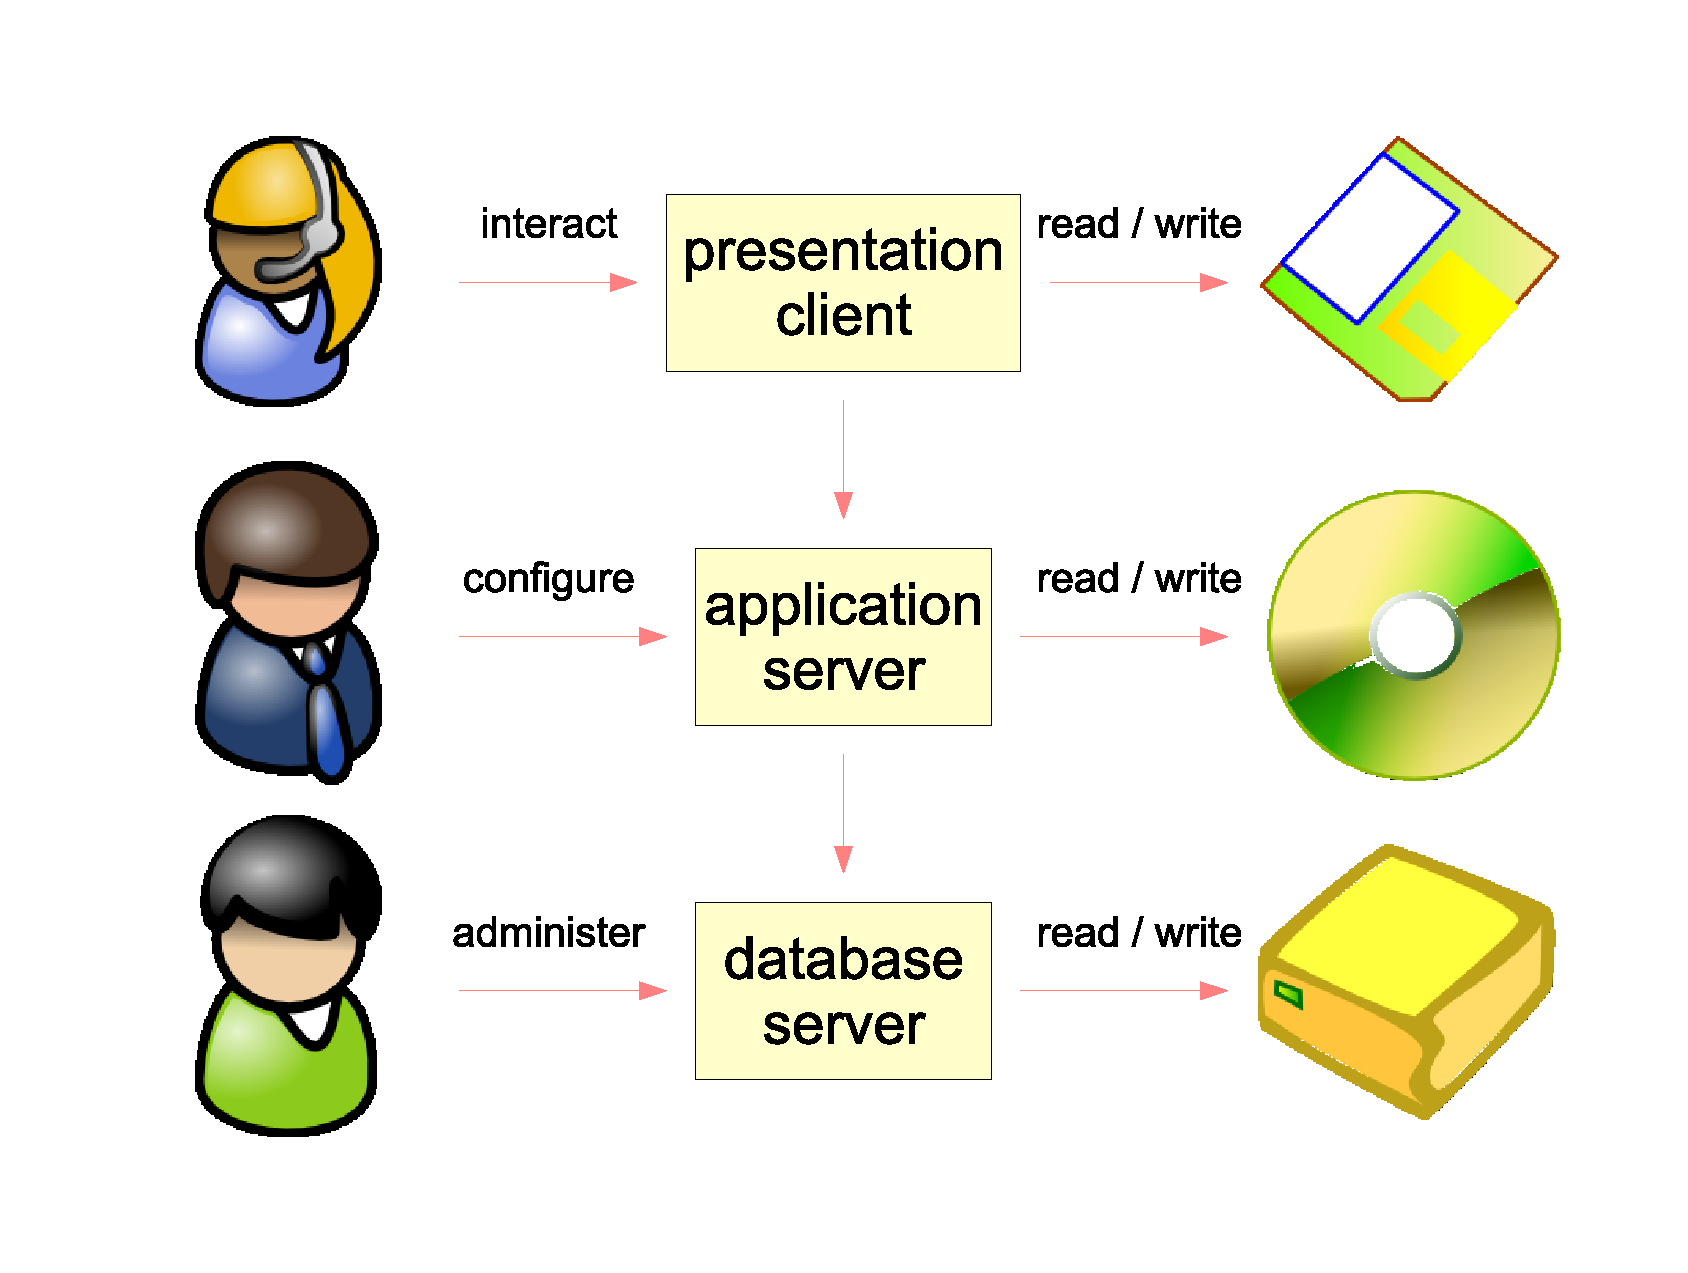
\includegraphics[scale=0.2]{vector/universal.eps}
        \caption{Universal Communication}
        \label{universal_figure}
    \end{center}
\end{figure}

Figure \ref{universal_figure} shows a three-tier environment: tier 1 represents
the \emph{Presentation Layer}; tier 2 stands for the \emph{Application Layer};
tier 3 is the \emph{Database (DB) Layer}. Typical synonyms are, in this order:
\emph{Frontend}, \emph{Business Logic} and \emph{Backend}. The tiers (layers)
serve two needs: connect different locations and share work load (\emph{Scaling}).
However, the split into tiers of that kind raises two illusions:

\begin{enumerate}
    \item \emph{Users only interact with clients}
    \item \emph{Persistent data are stored in DB only}
\end{enumerate}

Many IT architectures, or at least their illustrations, neglect the fact that
in reality \emph{all} systems need a \emph{User Interface} (UI), for at least
being administered by humans, and \emph{almost} all systems, even
\emph{Database Management Systems} (DBMS) themselves, store some of their
persistent data outside a database, for example locally available configuration
information. This is not necessarily a problem for the IT environment as such,
but it is for the internal architecture of software systems. Special solutions
have to deal with frontend (UI framework), business logic (domain patterns) and
backend (data mapping), and often additional mechanisms for local and remote
communication. The serious differences in these design solutions are one root
of well-known problems like multi- directional inter-dependencies between system
parts, that make software difficult to develop and hard to maintain.

One aim of the work described in this article was to investigate possibilities
for a \emph{unification} of communication paradigms, that is high-level design
paradigms rather than low-level protocols, in order to architect software in a
way that allows the computer system it runs on to communicate \emph{universally}.

%
% $RCSfile: modelling_mistakes.tex,v $
%
% Copyright (c) 2005-2006. Christian Heller. All rights reserved.
%
% Permission is granted to copy, distribute and/or modify this document
% under the terms of the GNU Free Documentation License, Version 1.1 or
% any later version published by the Free Software Foundation; with no
% Invariant Sections, with no Front-Cover Texts and with no Back-Cover
% Texts. A copy of the license is included in the section entitled
% "GNU Free Documentation License".
%
% http://www.cybop.net
% - Cybernetics Oriented Programming -
%
% http://www.resmedicinae.org
% - Information in Medicine -
%
% Version: $Revision: 1.1 $ $Date: 2006-01-03 08:21:45 $ $Author: christian $
% Authors: Christian Heller <christian.heller@tuxtax.de>
%

\subsection{Modelling Mistakes}
\label{modelling_mistakes_heading}

Most modern software is not written directly in a machine language but designed
in form of higher-level models instead. These allow to speed up application
development and help avoiding errors. \emph{Object Oriented Programming} (OOP),
for example, uses design concepts like the \emph{Class} owning \emph{Attributes}
and \emph{Methods}. Yet does this kind of modelling create abstractions that
reflect concepts of the real world completely and correctly?

\begin{figure}[ht]
    \begin{center}
        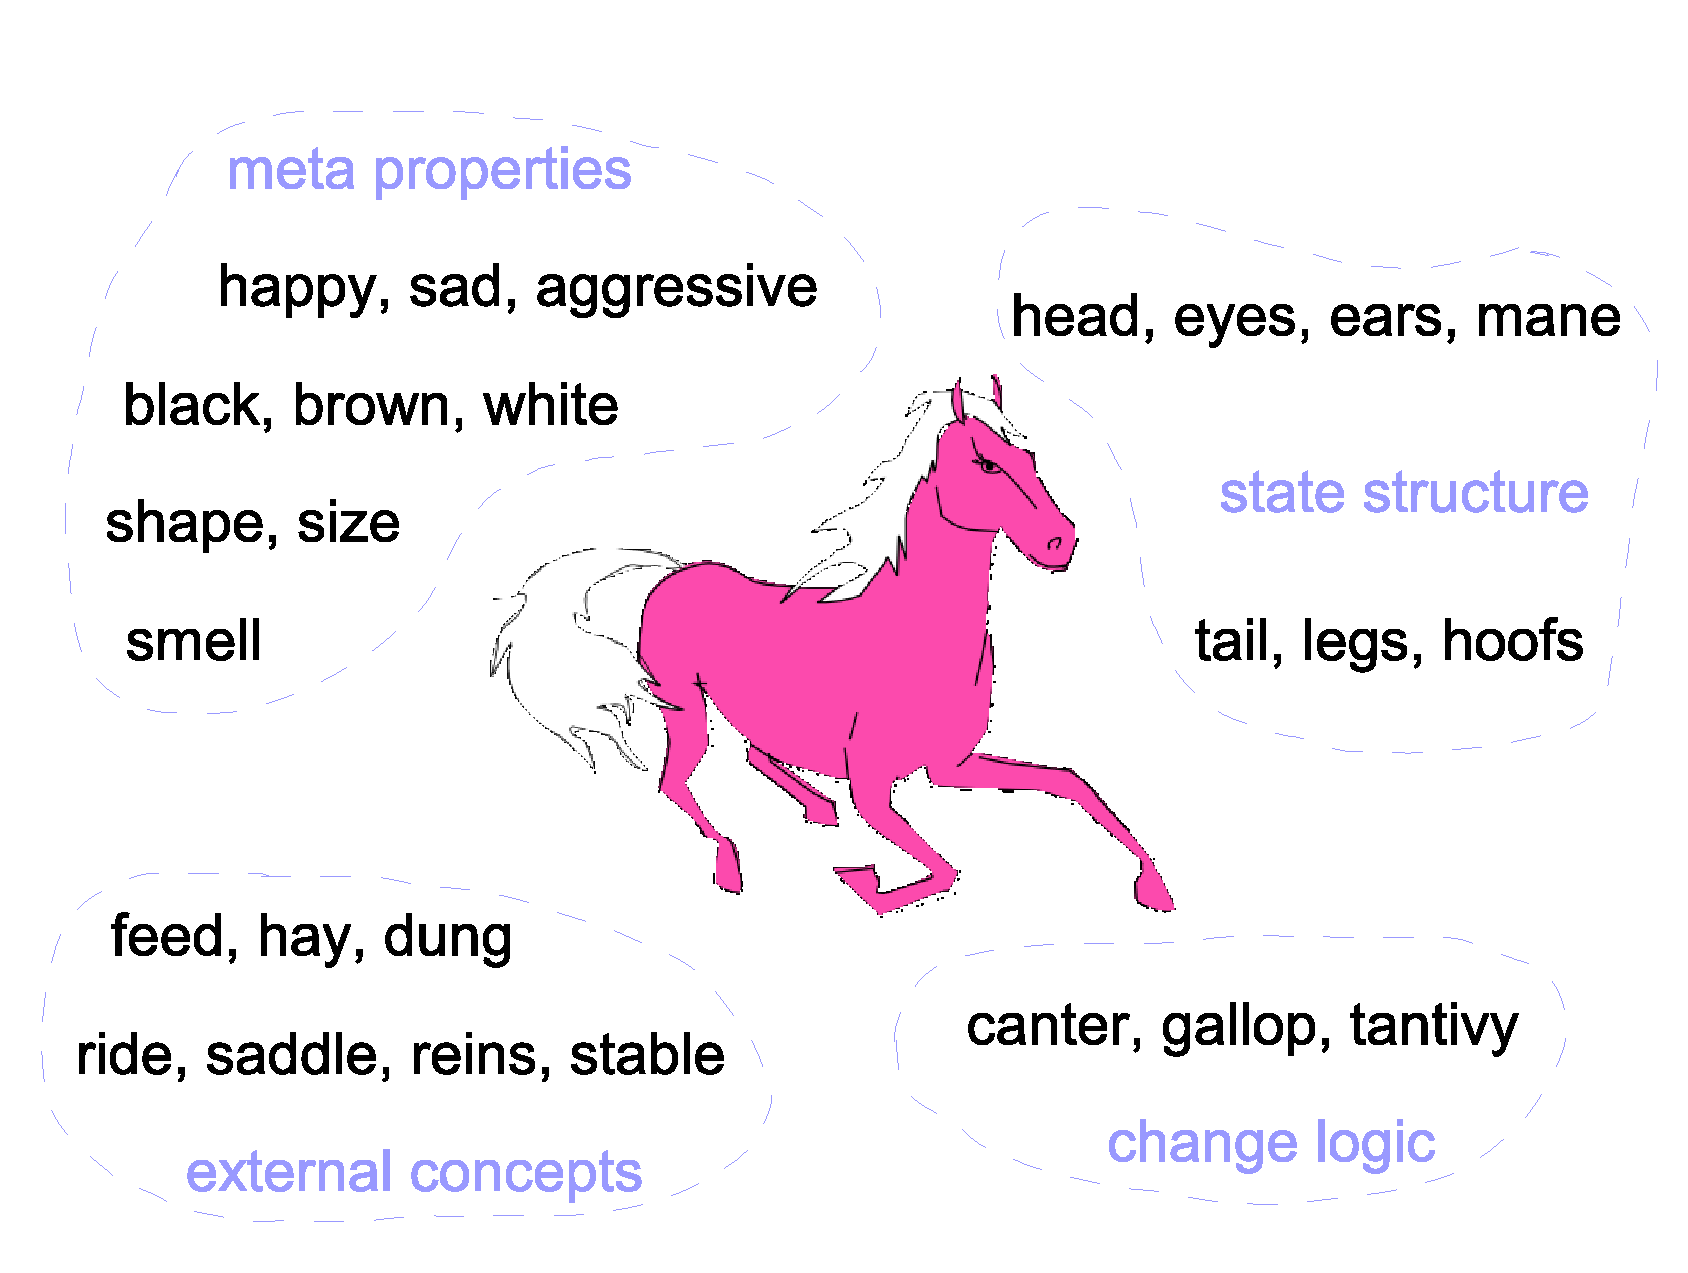
\includegraphics[scale=0.2]{vector/horse.eps}
        \caption{Concept of a Horse}
        \label{horse_figure}
    \end{center}
\end{figure}

The model of a \emph{Horse} shall serve as example to investigate this further.
Figure \ref{horse_figure} shows a number of terms commonly used to describe a
horse. Most importantly, there are structural observations describing the horse
as concept consisting of parts like \emph{Head}, \emph{Legs} or \emph{Hoofs}.
Secondly, there are properties like the horse's \emph{Colour}, \emph{Shape} or
\emph{Size}. Thirdly, there are terms describing a horse's actions like its
\emph{Movement} or \emph{Eating}, that change a horse's position and/ or state.
Finally, there are a number of terms like \emph{Hay} or \emph{Saddle}
associating concepts related to the horse.

One might suggest to model properties like the position, size or colour of a
horse's leg as \emph{Part} of that leg. In fact, this is how classical
programming approaches its solutions. In OOP, one would probably use a class
representing the leg and an attribute standing for the leg's colour. However,
when following the modelling principles of human thinking (see
\cite{heller2004}), this is \emph{not} correct!

It is true that in everyday language, one tends to say \textit{A horse leg
\emph{has a} colour.} Unfortunately, this leads to the wrong assumption that a
leg were made of a colour. But this is not the case. A leg does not
\emph{consist} of a colour in the hierarchical meaning of a whole consisting of
parts. The colour is rather property information \emph{about} the leg. It seems
there is no correct expression in natural (English) language stating the
property of something. The \emph{IS-A} verbalisation is used to express that
the leg belongs to a special category of items, for example: \textit{A leg is a
body element.} The \emph{HAS-A} formulation is used to express that a leg as
whole consists of smaller parts, for example: \textit{A leg has a knee and it
has a hoof.} But which formulation expresses a property? Well, perhaps it would
be best to say: \textit{A leg IS-OF a colour.}

The CYBOP knowledge schema described later in this article distinguishes
structural- from meta information. Actions (like the gallop of a horse) causing
change in the model or its environment are called \emph{Logic} in this work,
since they follow certain rules.


    %
% $RCSfile: basic_patterns.tex,v $
%
% Copyright (c) 2001-2004. Christian Heller. All rights reserved.
%
% No copying, altering, distribution or any other actions concerning this
% document, except after explicit permission by the author!
% At some later point in time, this document is planned to be put under
% the GNU FDL license. For now, _everything_ is _restricted_ by the author.
%
% http://www.cybop.net
% - Cybernetics Oriented Programming -
%
% http://www.resmedicinae.org
% - Information in Medicine -
%
% @author Christian Heller <christian.heller@tuxtax.de>
%

\section{Basic Patterns}
\label{basic_patterns_heading}

%
% $RCSfile: data_mapper.tex,v $
%
% Copyright (c) 2004. Christian Heller. All rights reserved.
%
% No copying, altering, distribution or any other actions concerning this
% document, except after explicit permission by the author!
% At some later point in time, this document is planned to be put under
% the GNU FDL license. For now, _everything_ is _restricted_ by the author.
%
% http://www.cybop.net
% - Cybernetics Oriented Programming -
%
% http://www.resmedicinae.org
% - Information in Medicine -
%
% @author Christian Heller <christian.heller@tuxtax.de>
%

\paragraph{Data Mapper}
\label{data_mapper_heading}

Besides the \emph{Domain Logic}, standard three-tier architectures contain a
\emph{Data Source} layer which may for example represent a database. Both layers
need to exchange data. Modern systems use OOP methods to implement the domain
model. Database models, on the other hand, are often implemented as
\emph{Entity Relationship Model} (ERM).

In order to avoid close coupling and a mix-up of both layers, the introduction
of an additional \emph{Data Mapper} layer \cite{fowler2002} in between the two
others may be justified (figure \ref{datamapper_figure}). The most important
idea of this pattern is to abolish the interdependencies of domain- and
persistence model (database).

\begin{figure}[ht]
    \begin{center}
        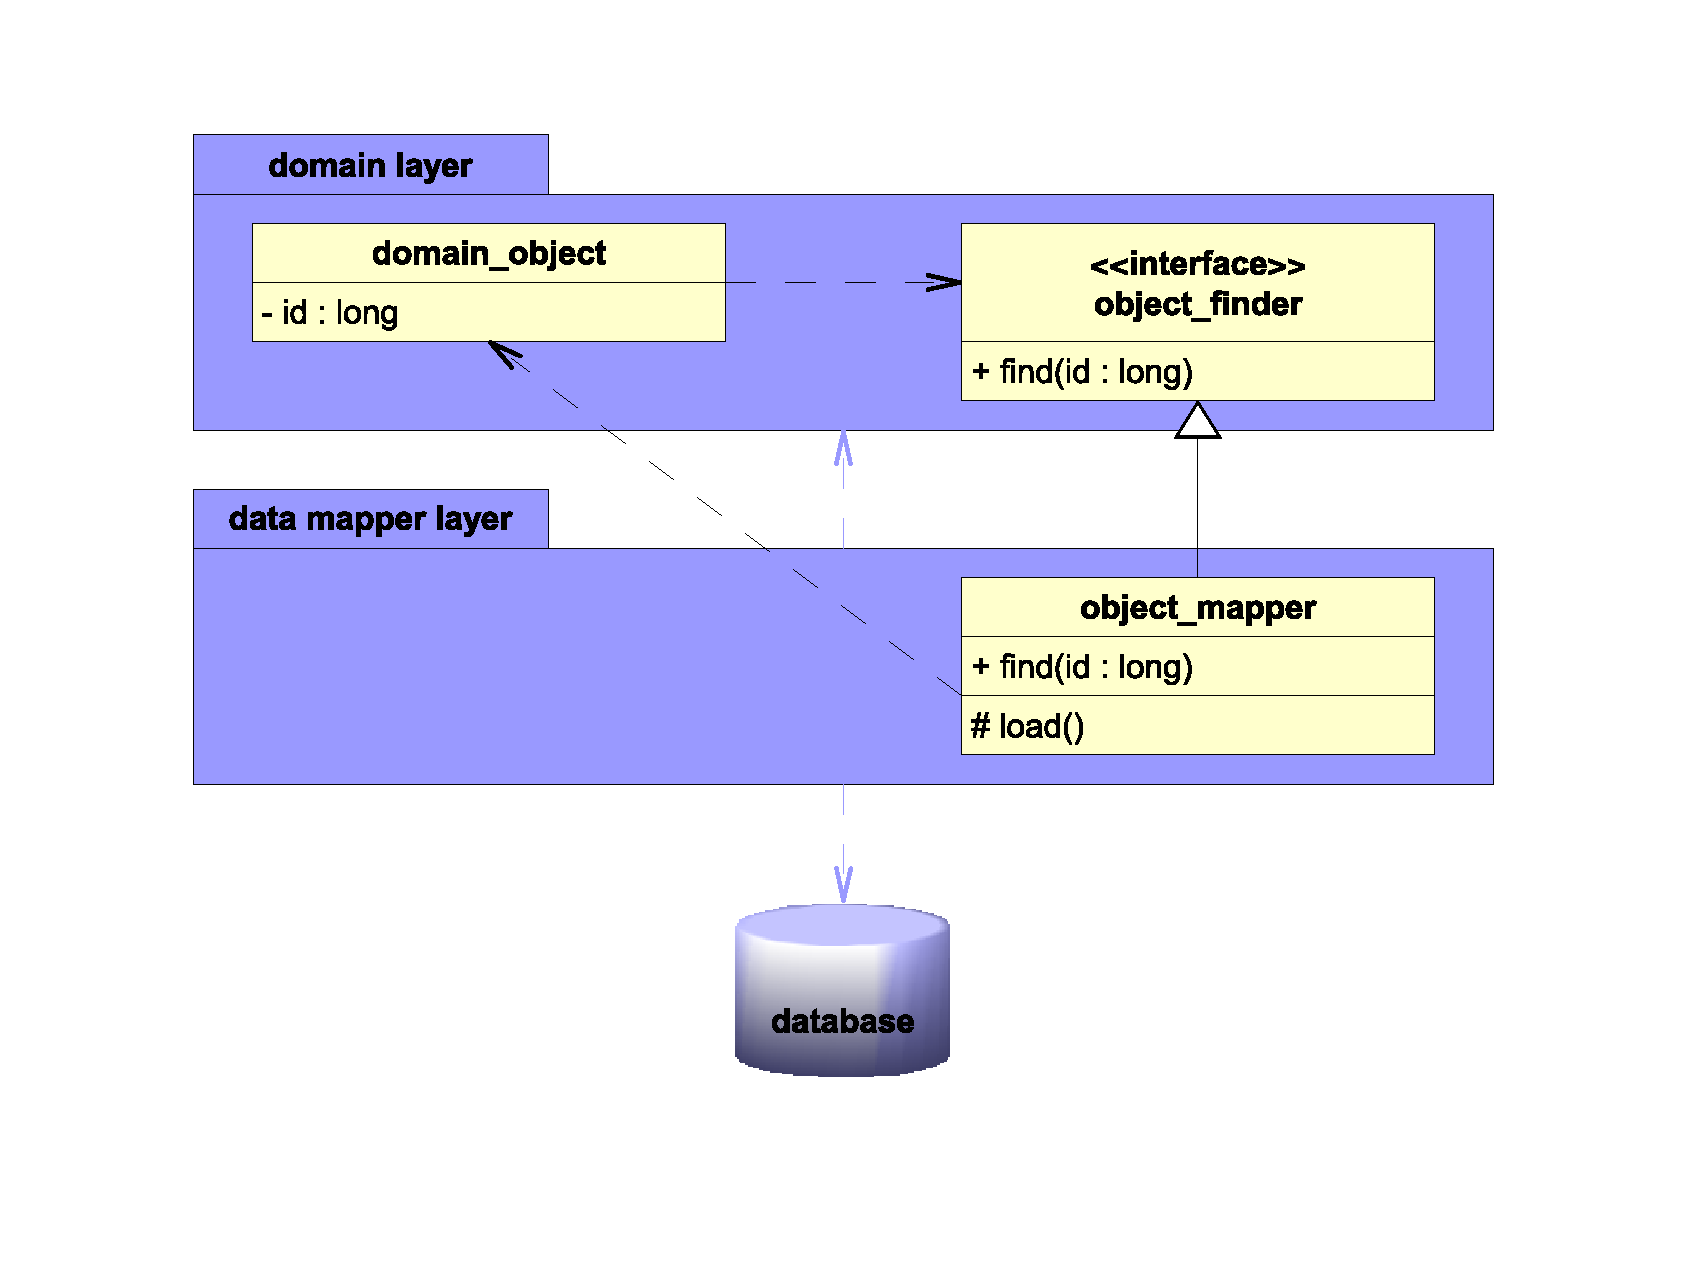
\includegraphics[scale=0.3]{vector/datamapper.eps}
        \caption{Data Mapper Pattern}
        \label{datamapper_figure}
    \end{center}
\end{figure}

The dashed arrows in figure \ref{datamapper_figure} indicate dependencies. The
data mapper layer knows the domain model- as well as the data source layer, via
\emph{unidirectional} relations. Its task is to \emph{translate} between the two,
in both directions. Domain model and data source know nothing from each other.

Each domain model class knows its appropriate interface (\emph{object\_finder})
but does not know the implementation of the same. That is, persistence- and
data retrieval mechanisms are hidden in front of the domain model. The
implementation (\emph{object\_mapper}) is part of the mapping package and also
implements all finder methods. It maps data of the received result sets to the
special attributes of the domain model objects.

The \emph{Mediator} pattern \cite{gamma1995} is similar to the \emph{Mapper}, in
that it is used to decouple different parts of a system. Fowler \cite{fowler2002}
writes: \textit{\ldots the objects that use a mediator are aware of it, even if
they aren't aware of each other; the objects that a mapper separates aren't even
aware of the mapper.}

Although the \emph{Data Mapper} pattern is very helpful at implementing OO
systems, two things are to be criticised:

Firstly, since the \emph{object\_finder} relies on functionality specific to the
retrieval of persistent data, it does actually belong into the data mapper layer
what, if done, would create bidirectional dependencies between the domain model-
and data mapper layer. But also with the \emph{object\_finder} remaining in the
domain model layer, dependencies are not purely unidirectional. It is true that
from an OO view, they are. Internally, however, a super class or interface
relates to its inheriting classes, so that it can call their methods to satisfy
the polymorphic behaviour.

Secondly, the layers do not truely build on each other. Taken a standard
architecture consisting of the following five -- instead of only three -- layers:

\begin{enumerate}
    \item Presentation
    \item Application Process
    \item Domain Model
    \item Data Mapper
    \item Data Source
\end{enumerate}

\ldots the application process does not only access the domain model layer, it
also has to manage (create and destroy) the objects of the data mapper layer.
In other words, it surpasses (disregards) the domain model layer when accessing
the data mapper layer directly.

%
% $RCSfile: data_transfer_object.tex,v $
%
% Copyright (c) 2004. Christian Heller. All rights reserved.
%
% No copying, altering, distribution or any other actions concerning this
% document, except after explicit permission by the author!
% At some later point in time, this document is planned to be put under
% the GNU FDL license. For now, _everything_ is _restricted_ by the author.
%
% http://www.cybop.net
% - Cybernetics Oriented Programming -
%
% http://www.resmedicinae.org
% - Information in Medicine -
%
% @author Christian Heller <christian.heller@tuxtax.de>
%

\paragraph{Data Transfer Object}
\label{data_transfer_object_heading}

It is a well-known fact that many small requests between two processes, and
even more between two hosts in a network need a lot of time. A local machine
with two processes has to permanently change the \emph{Program Context}; a
network has a lot of \emph{Transfers}. For each request, there is a necessity
of at least \emph{two} transfers -- the \emph{Question} of the client and the
\emph{Answer} of the server.

Transfer methods are often expected to deliver common data such as a Person's
address, that is surname, first name, street, zip-code, town and so on. These
information is best retrieved by only \emph{one} transfer call. That way, the
client has to wait only once for a server response and the server does not get
too many single tasks. In this example, all address data would best be packaged
together and sent back to the client.

\begin{figure}[ht]
    \begin{center}
       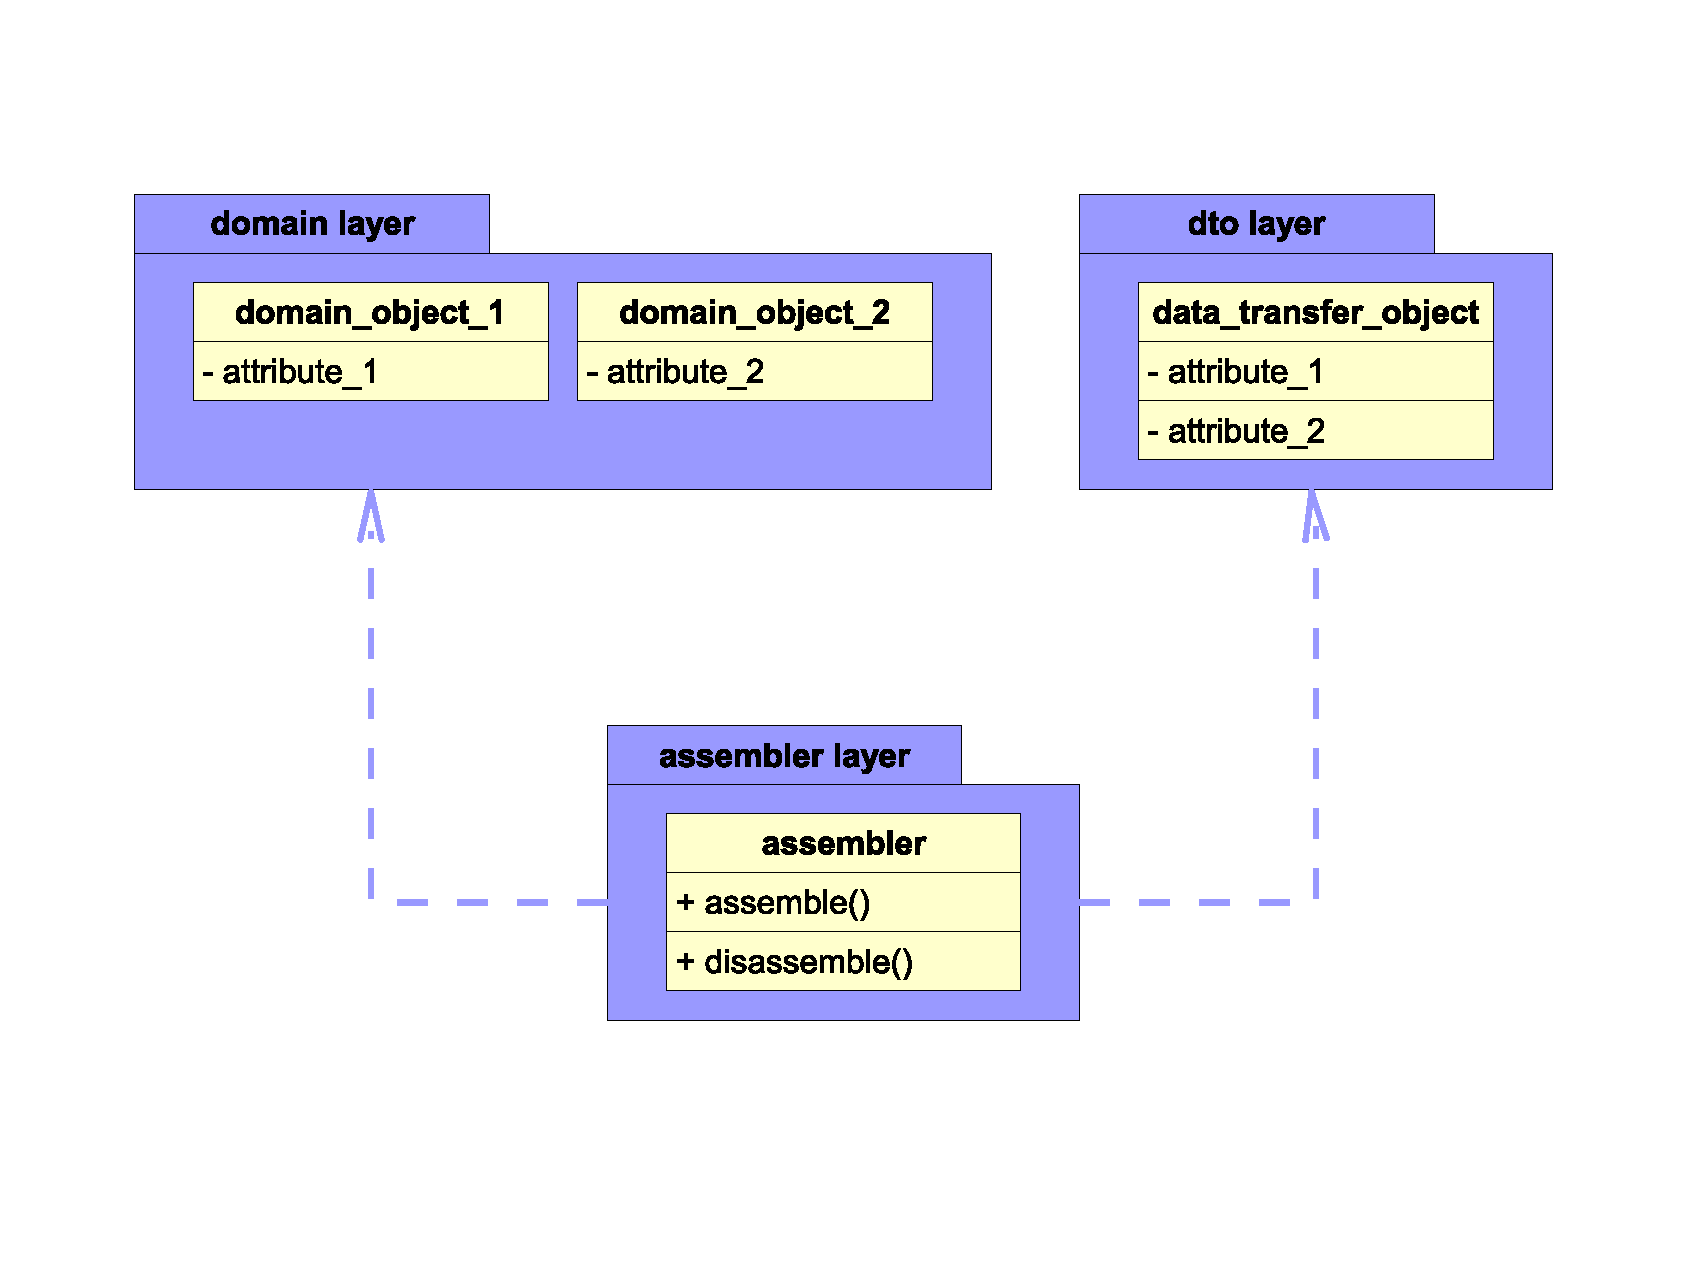
\includegraphics[scale=0.3]{vector/dto.eps}
       \caption{Data Transfer Object Pattern}
       \label{dto_figure}
    \end{center}
\end{figure}

A scenario of that kind is exactly what the \emph{Data Transfer Object} pattern
\cite{fowler2002} proposes a solution for: A central \emph{Assembler} object
takes all common data of the server's domain model objects and assembles them
together into a special \emph{Data Transfer Object} (DTO), which is a flat data
structure (figure \ref{dto_figure}). The server will then send this DTO over
network to the client. On the client's side, a similar assembler takes the DTO,
finds out all received data and maps (disassembles) them to the client's domain
model. In that manner, a DTO is able to drastically improve the communication
performance.

%
% $RCSfile: model_view_controller.tex,v $
%
% Copyright (C) 2002-2008. Christian Heller.
%
% Permission is granted to copy, distribute and/or modify this document
% under the terms of the GNU Free Documentation License, Version 1.1 or
% any later version published by the Free Software Foundation; with no
% Invariant Sections, with no Front-Cover Texts and with no Back-Cover
% Texts. A copy of the license is included in the section entitled
% "GNU Free Documentation License".
%
% http://www.cybop.net
% - Cybernetics Oriented Programming -
%
% http://www.resmedicinae.org
% - Information in Medicine -
%
% Version: $Revision: 1.1 $ $Date: 2008-08-19 20:41:07 $ $Author: christian $
% Authors: Christian Heller <christian.heller@tuxtax.de>
%

\subsubsection{Model View Controller}
\label{model_view_controller_heading}
\index{Model View Controller Pattern}
\index{MVC}
\index{Graphical User Interface}
\index{GUI}
\index{Observer Pattern}
\index{Strategy Pattern}
\index{Wrapper Pattern}
\index{Composite Pattern}
\index{Java Foundation Classes}
\index{JFC}
\index{Microsoft Foundation Classes}
\index{MFC}
\index{Document View MVC Variant}
\index{Translator Architecture}

After having had a closer look at design patterns for persistence
(\emph{Data Mapper}) and communication (\emph{Data Transfer Object}), this
section considers the presentation layer of an application (figure
\ref{logical_figure}), which is often realised in form of a
\emph{Graphical User Interface} (GUI). Nowadays, the well-known
\emph{Model View Controller} (MVC) pattern \cite{buschmann, fowler2002} is used
by a majority of standard business applications. Its principle is to have the
\emph{Model} holding domain data, the \emph{View} accessing and displaying
these data and the \emph{Controller} providing the workflow of the application
by handling any action events happening on the view (figure \ref{mvc_figure}).
This separation eases the creation of applications with many synchronous views
on the same data. Internally, the MVC may consist of design patterns like:

\begin{figure}[ht]
    \begin{center}
        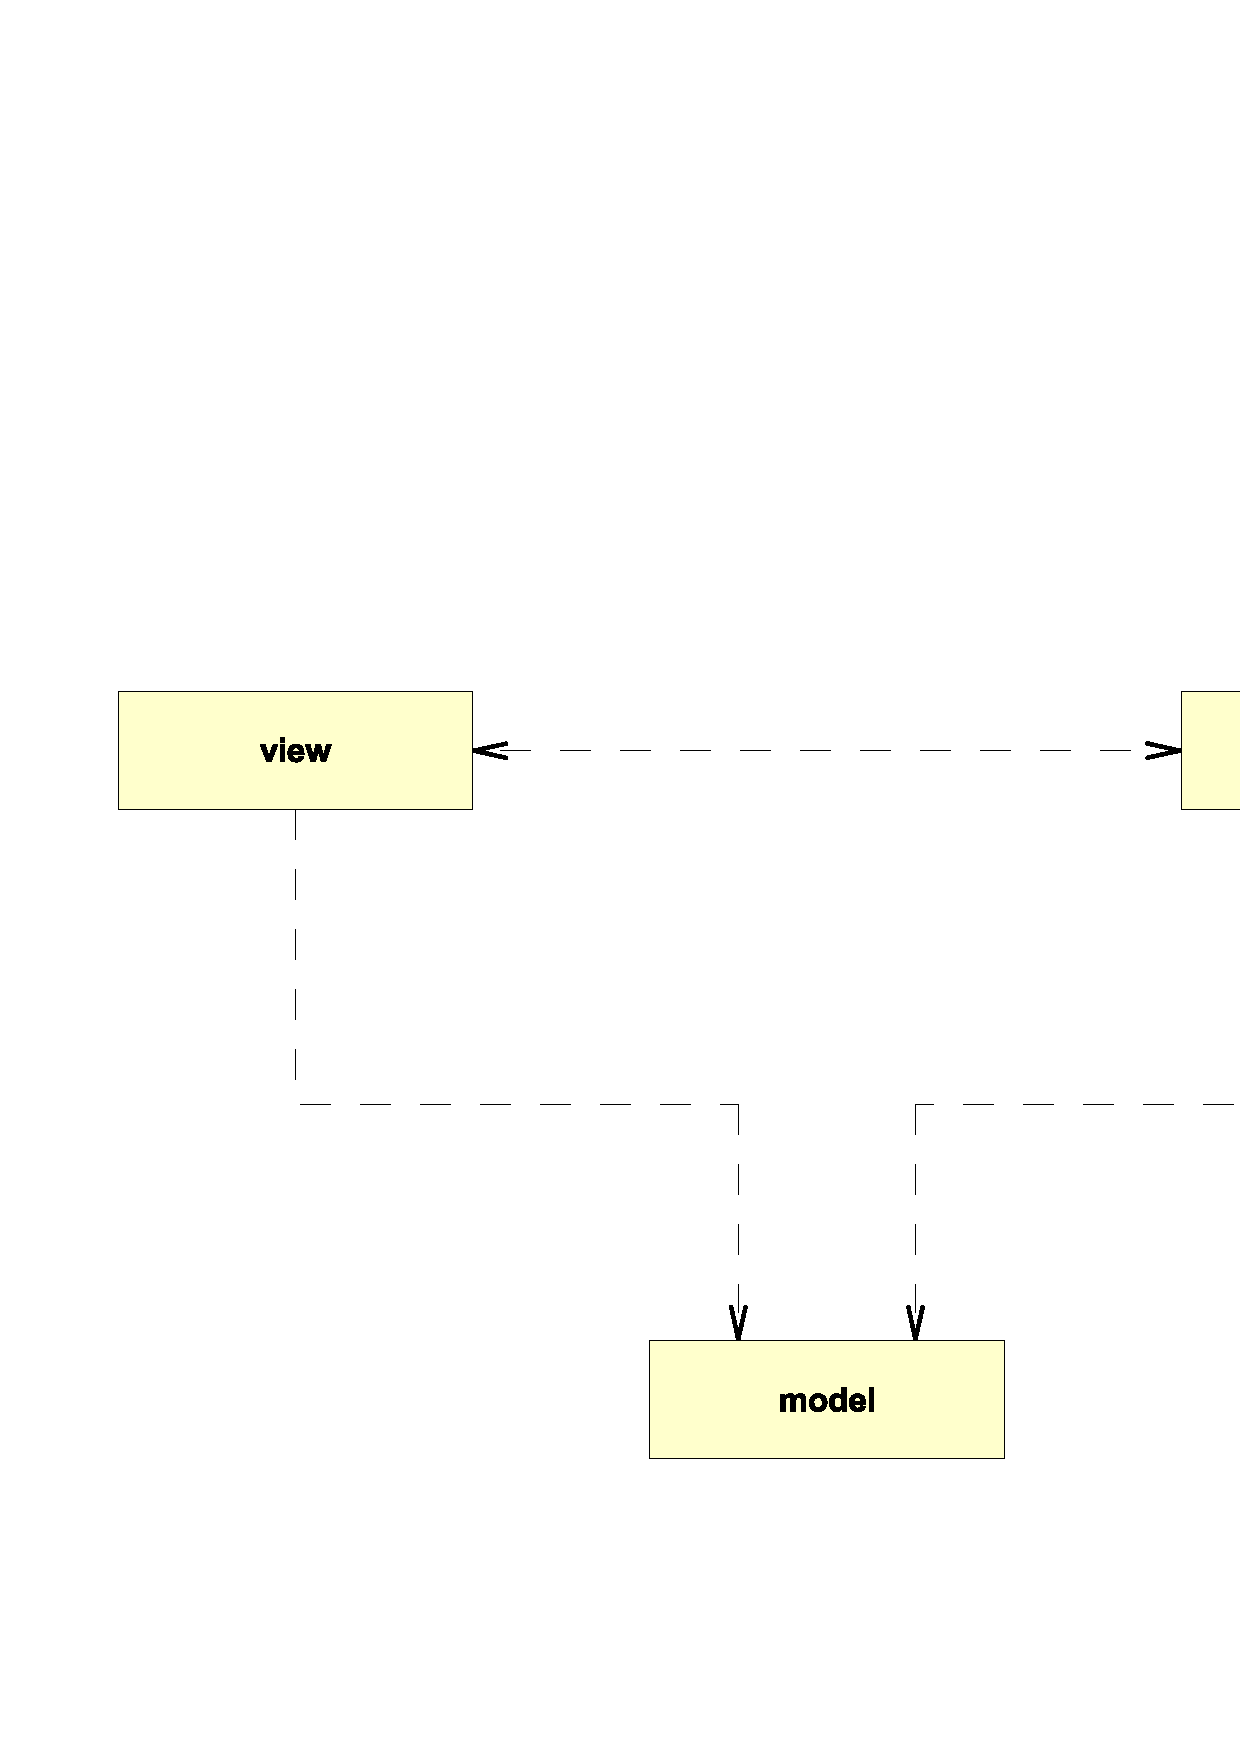
\includegraphics[scale=0.3,angle=-90]{graphic/mvc.pdf}
        \caption{Model View Controller Pattern}
        \label{mvc_figure}
    \end{center}
\end{figure}

\begin{itemize}
    \item[-] \emph{Observer} (section \ref{observer_heading}) which notifies
        the views about data model changes
    \item[-] \emph{Strategy} \cite{gamma1995} which encapsulates exchangeable
        functionality of the controller
    \item[-] \emph{Wrapper} (section \ref{wrapper_heading}) which delegates
        controller functionality to the \emph{Strategy}
    \item[-] \emph{Composite} (section \ref{composite_heading}) which equips
        graphical views with a hierarchical structure
\end{itemize}

Some MVC implementations like parts of the \emph{Java Foundation Classes} (JFC)
use a simplified version not separating controllers from their views. The
\emph{Microsoft Foundation Classes} (MFC) C++ library calls its implementation
\emph{Document-View}.

Besides the above-mentioned patterns \emph{Data Mapper} and DTO, MVC is the
third one getting merged into a common \emph{Translator} architecture, in
chapter \ref{state_and_logic_heading}.



    %
% $RCSfile: hierarchy_and_ontology.tex,v $
%
% Copyright (c) 2001-2004. Christian Heller. All rights reserved.
%
% No copying, altering, distribution or any other actions concerning this
% document, except after explicit permission by the author!
% At some later point in time, this document is planned to be put under
% the GNU FDL license. For now, _everything_ is _restricted_ by the author.
%
% http://www.cybop.net
% - Cybernetics Oriented Programming -
%
% http://www.resmedicinae.org
% - Information in Medicine -
%
% @author Christian Heller <christian.heller@tuxtax.de>
%

\section{Hierarchy and Ontology}
\label{hierarchy_and_ontology_heading}

Section \ref{basic_patterns_heading} explained three design patterns that are
widely used in software architectures. It has shown similarities between them
and raised the question if they could possibly be merged into just one pattern,
called \emph{Translator}, what will be described in section
\ref{logical_architecture_heading}.
Yet before, this section will demonstrate how the principle of \emph{Hierarchy}
may be applied to obtain an \emph{Ontology}.

%
% $RCSfile: association_elimination.tex,v $
%
% Copyright (c) 2001-2004. Christian Heller. All rights reserved.
%
% No copying, altering, distribution or any other actions concerning this
% document, except after explicit permission by the author!
% At some later point in time, this document is planned to be put under
% the GNU FDL license. For now, _everything_ is _restricted_ by the author.
%
% http://www.cybop.net
% - Cybernetics Oriented Programming -
%
% http://www.resmedicinae.org
% - Information in Medicine -
%
% @author Christian Heller <christian.heller@tuxtax.de>
%

\subsection{Association Elimination}
\label{association_elimination_heading}

An \emph{Electronic Health Record} (EHR) will serve as example domain model whose class
structure is shown in part in figure \ref{parent_eliminate_child_associations_figure}.
It consists of numerous parts whereof at least two will be of type \emph{Address}
and \emph{Problem}, respectively. Following the \emph{Episode-based EHR}
recommendation \cite{westerhof}, \emph{Problem} may consist of \emph{Subjective}
and \emph{Objective}. All these associations between classes are needed to
navigate through the domain model.

\begin{figure}[ht]
    \begin{center}
        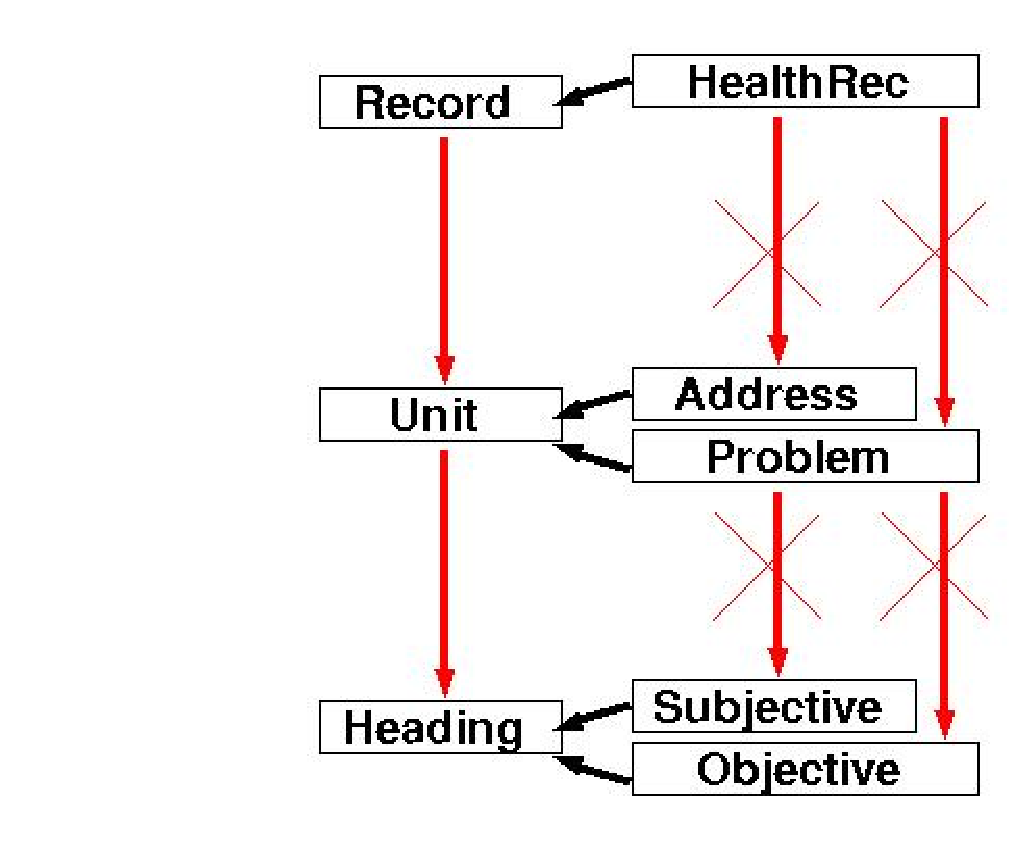
\includegraphics[scale=0.4]{vector/parent_eliminate_child_associations.eps}
        \caption{Parent- eliminate Child Associations}
        \label{parent_eliminate_child_associations_figure}
    \end{center}
\end{figure}

A frequent design decision in object oriented programming is to sum up common
properties of sub classes by introducing a common super class. It is not only
properties, but also the \emph{Granularity} of objects that can lead to the
creation of a super class. The OpenEHR project \cite{openehr} suggests to let
the above-mentioned classes inherit from the more coarse-grained super classes
\emph{Record}, \emph{Unit}, \emph{Heading} and others.\\
Whichever reason -- once the super classes are there, they should be associated
similarly to their sub classes, that is in the same direction, using unidirectional
dependencies. Afterwards, all associations between sub classes become superfluous
as every sub class can reach its sibling across their parent classes' association
(figure \ref{parent_eliminate_child_associations_figure}).\\
Here a short Java code example for how the \emph{HealthRecord} may retrieve a
reference to \emph{Address}:
\begin{verbatim}
Address a = (Address) get("address");
\end{verbatim}
\emph{HealthRecord} inherits the \emph{get} method from its super class \emph{Record}.
\emph{Record} holds many instances of type \emph{Unit} and differing sub types.
The \emph{get} method delivers back an object that still needs to be down-casted
to the expected sub type \emph{Address}.\\
The definition of classes, their dependencies (defined by associations) and granularities
(defined by inheritance) in a software system results in several layers of classes of
common granularity, as shown in figure \ref{ontological_levels_and_item_container_figure}.
These layers are often called \emph{Ontological Level} as they form an \emph{Ontology}
(see section \ref{ontology_heading}).

\begin{figure}[ht]
    \begin{center}
        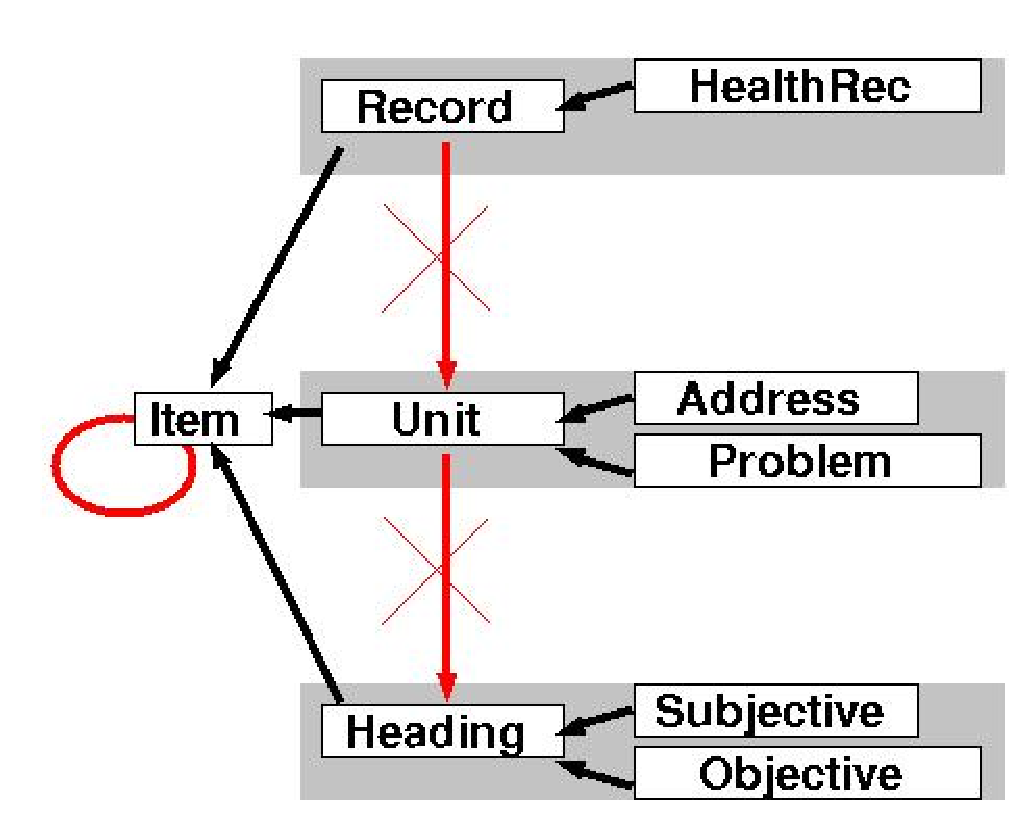
\includegraphics[scale=0.4]{vector/ontological_levels_and_item_container.eps}
        \caption{Ontological Levels and Item Container}
        \label{ontological_levels_and_item_container_figure}
    \end{center}
\end{figure}

Continuing the structure process of introducing more and more common, coarse-grained
or fine-grained super classes, the development culminates in one top-most super
class of all other classes in the system, which this paper calls \emph{Item}.
It is as general as the \emph{java.lang.Object} class for the Java class library,
only that it additionally represents a container that can store objects of any type,
as explained in \cite{hellerbohl}. In other words, \emph{Item} provides the meta
functionality of a container behaviour to \emph{all} other classes.


%
% $RCSfile: ontology.tex,v $
%
% Copyright (c) 2001-2004. Christian Heller. All rights reserved.
%
% No copying, altering, distribution or any other actions concerning this
% document, except after explicit permission by the author!
% At some later point in time, this document is planned to be put under
% the GNU FDL license. For now, _everything_ is _restricted_ by the author.
%
% http://www.cybop.net
% - Cybernetics Oriented Programming -
%
% http://www.resmedicinae.org
% - Information in Medicine -
%
% @author Christian Heller <christian.heller@tuxtax.de>
%

\subsection{Ontology}
\label{ontology_heading}

Manifold definitions of the word \emph{Ontology} exist. They come from philosophy,
metaphysics, information technology and others -- too many to list here.
This document uses its own, adapted definition and considers an ontology to be
\emph{a strict hierarchy of abstract items, organized in levels of growing
granularity, that are solely unidirectionally related}. It such represents a
systematic description of complex domain contexts.

\begin{figure}[ht]
    \begin{center}
        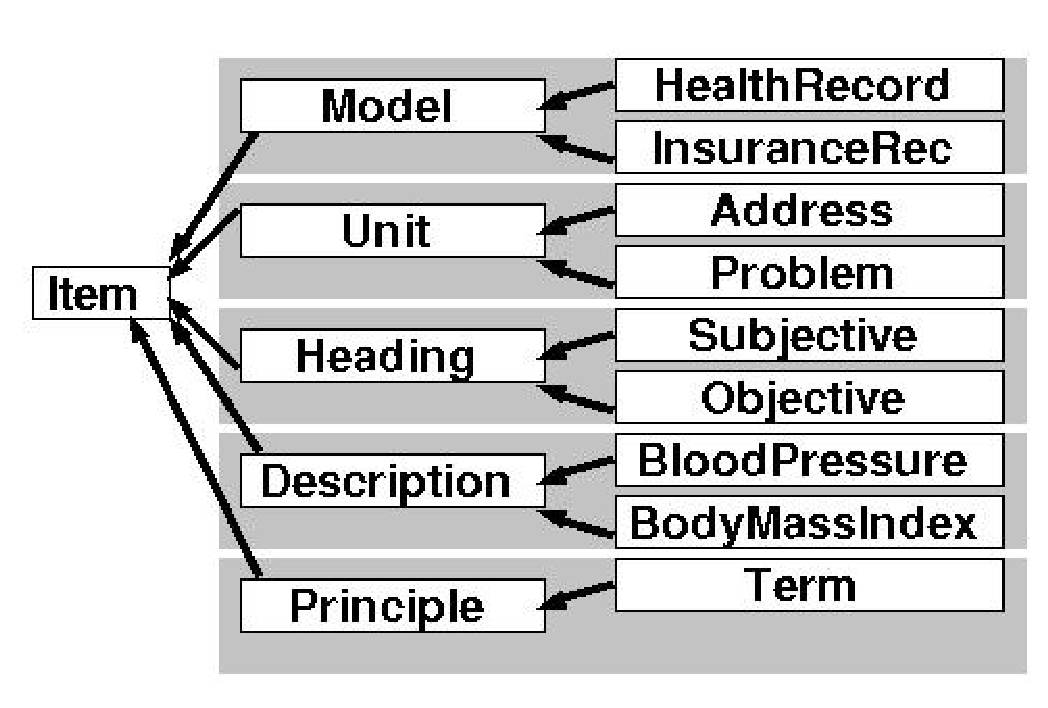
\includegraphics[scale=0.4]{vector/electronic_health_record_ontology.eps}
        \caption{Electronic Health Record Ontology}
        \label{electronic_health_record_ontology_figure}
    \end{center}
\end{figure}

Figure \ref{electronic_health_record_ontology_figure} shows one possible ontology
of an electronic health record, as described in the previous section.




    %
% $RCSfile: logical_architecture.tex,v $
%
% Copyright (c) 2001-2004. Christian Heller. All rights reserved.
%
% No copying, altering, distribution or any other actions concerning this
% document, except after explicit permission by the author!
% At some later point in time, this document is planned to be put under
% the GNU FDL license. For now, _everything_ is _restricted_ by the author.
%
% http://www.cybop.net
% - Cybernetics Oriented Programming -
%
% http://www.resmedicinae.org
% - Information in Medicine -
%
% @author Christian Heller <christian.heller@tuxtax.de>
%

\section{Logical Architecture}
\label{logical_architecture_heading}

This section will sort the design patterns of section \ref{basic_patterns_heading}
into the layered architecture of a standard application. Afterwards, the
hierarchical principles of section \ref{hierarchy_and_ontology_heading} are applied
to simplify and merge the design patterns which will lead to an ontology.

\begin{figure}[ht]
    \begin{center}
        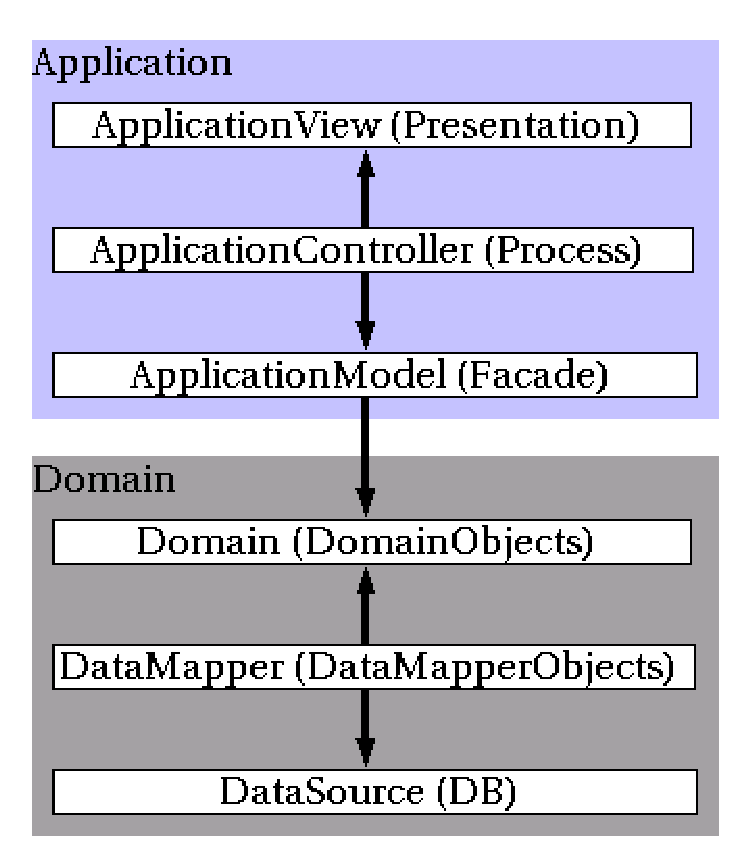
\includegraphics[scale=0.3]{vector/layered_architecture.eps}
        \caption{Layered Architecture}
        \label{layered_architecture_figure}
    \end{center}
\end{figure}

A state-of-the-art software system consists of a layered architecture similar to the
one shown in figure \ref{layered_architecture_figure}. The startable \emph{Controller}
process creates the whole application tree, to which belong the \emph{View} (as
user interface), the \emph{Model} (providing data to the view and as facade to
remote servers) and the \emph{Domain} with its database \emph{Mapper} layer.\\
It is not difficult to figure out where the basic patterns of section \ref{basic_patterns_heading}
fit in here (figure \ref{layered_architecture_with_basic_patterns_figure}):
The \emph{Model View Controller} pattern determines the classes to interact with
a human user via the \emph{View} (sometimes called \emph{Presentation Layer});
the \emph{Data Mapper} pattern provides necessary classes and an \emph{Entity
Relationship Model} (ERM) to connect to a persistence medium such as a database;
the \emph{Data Transfer Object} (DTO) pattern, finally, serves as means of
communication with remote servers.

\begin{figure}[ht]
    \begin{center}
        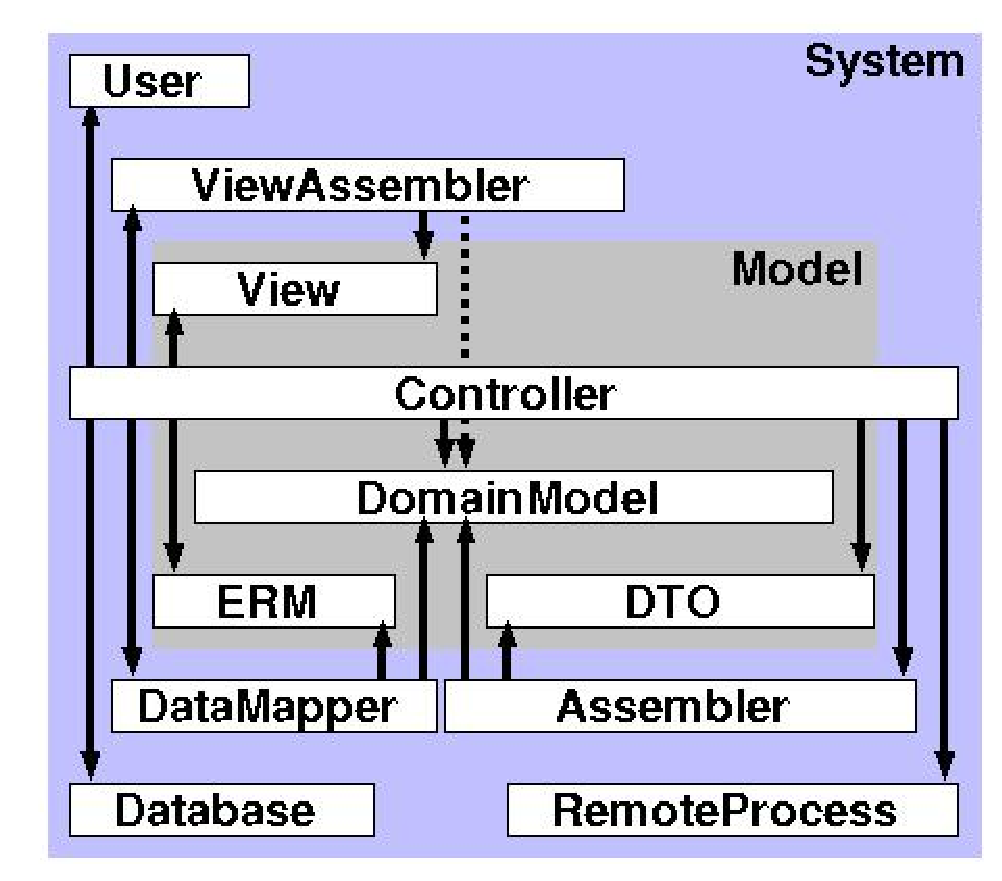
\includegraphics[scale=0.3]{vector/layered_architecture_with_basic_patterns.eps}
        \caption{Layered Architecture with Basic Patterns}
        \label{layered_architecture_with_basic_patterns_figure}
    \end{center}
\end{figure}

For all three kinds of communication, there is a:
\begin{itemize}
    \item[-] System (HumanUser, DataBase, RemoteServer)
    \item[-] Model (View, ERM, DTO)
    \item[-] Translator (ViewAssembler, Mapper, DTOAssembler)
\end{itemize}

Realizing this, it is easy to create ontological layers by adding one common
parent class for systems, models and translators each, which leads to a much
clearer architecture (figure \ref{layered_architecture_with_merged_patterns_figure}).
The common properties of all sub classes are merged into their corresponding super
class.

\begin{figure}[ht]
    \begin{center}
        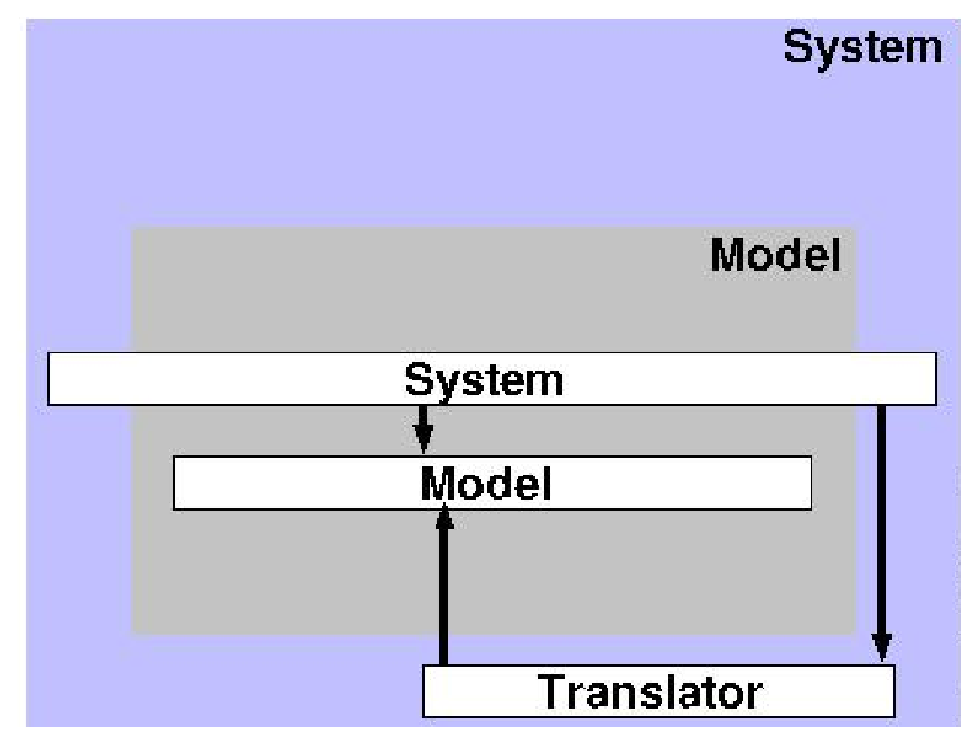
\includegraphics[scale=0.3]{vector/layered_architecture_with_merged_patterns.eps}
        \caption{Layered Architecture with merged Patterns}
        \label{layered_architecture_with_merged_patterns_figure}
    \end{center}
\end{figure}


    %
% $RCSfile: biological_reflections.tex,v $
%
% Copyright (c) 2001-2004. Christian Heller. All rights reserved.
%
% No copying, altering, distribution or any other actions concerning this
% document, except after explicit permission by the author!
% At some later point in time, this document is planned to be put under
% the GNU FDL license. For now, _everything_ is _restricted_ by the author.
%
% http://www.cybop.net
% - Cybernetics Oriented Programming -
%
% http://www.resmedicinae.org
% - Information in Medicine -
%
% @author Christian Heller <christian.heller@tuxtax.de>
%

\section{Biological Reflections}
\label{biological_reflections_heading}

The previous sections have shown how existing patterns for communication can be
merged into one common system architecture. All of these design patterns suggest
their very own communication paradigm which cannot be used anymore in the new,
merged \emph{Translator} architecture. Therefore, a new way for system interaction
needs to be found.

\begin{figure}[ht]
    \begin{center}
        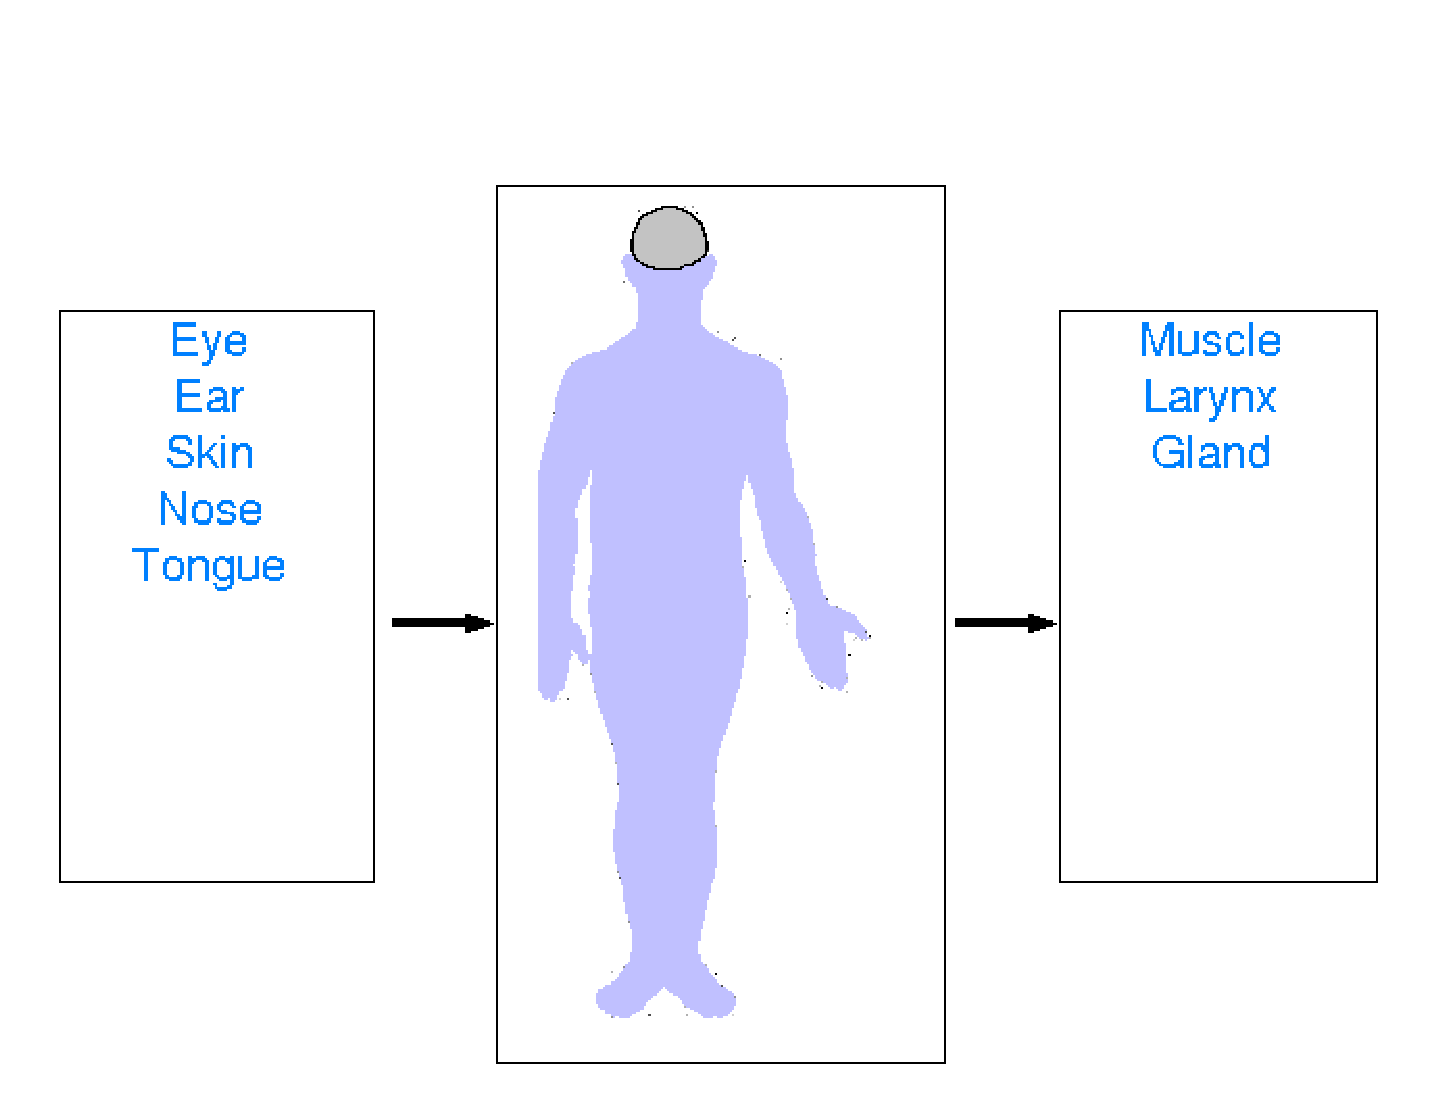
\includegraphics[scale=0.3]{vector/human_being_as_system.eps}
        \caption{Human Being as System of Models (Brain)}
        \label{human_being_as_system_figure}
    \end{center}
\end{figure}

Following the CYBOP approach, nature -- in our case the Human body -- will be
considered next. Humans have organs responsible for information input and output
(figure \ref{human_being_as_system_figure}). In between input and output, the
information is processed by the brain that contains a specific abstract model
of the surrounding real world. The human brain consists of several regions, each
being responsible for a special task, such as the optical region for seeing or the
cerebral cortex for actual information processing which possibly leads to awareness.

\begin{figure}[ht]
    \begin{center}
        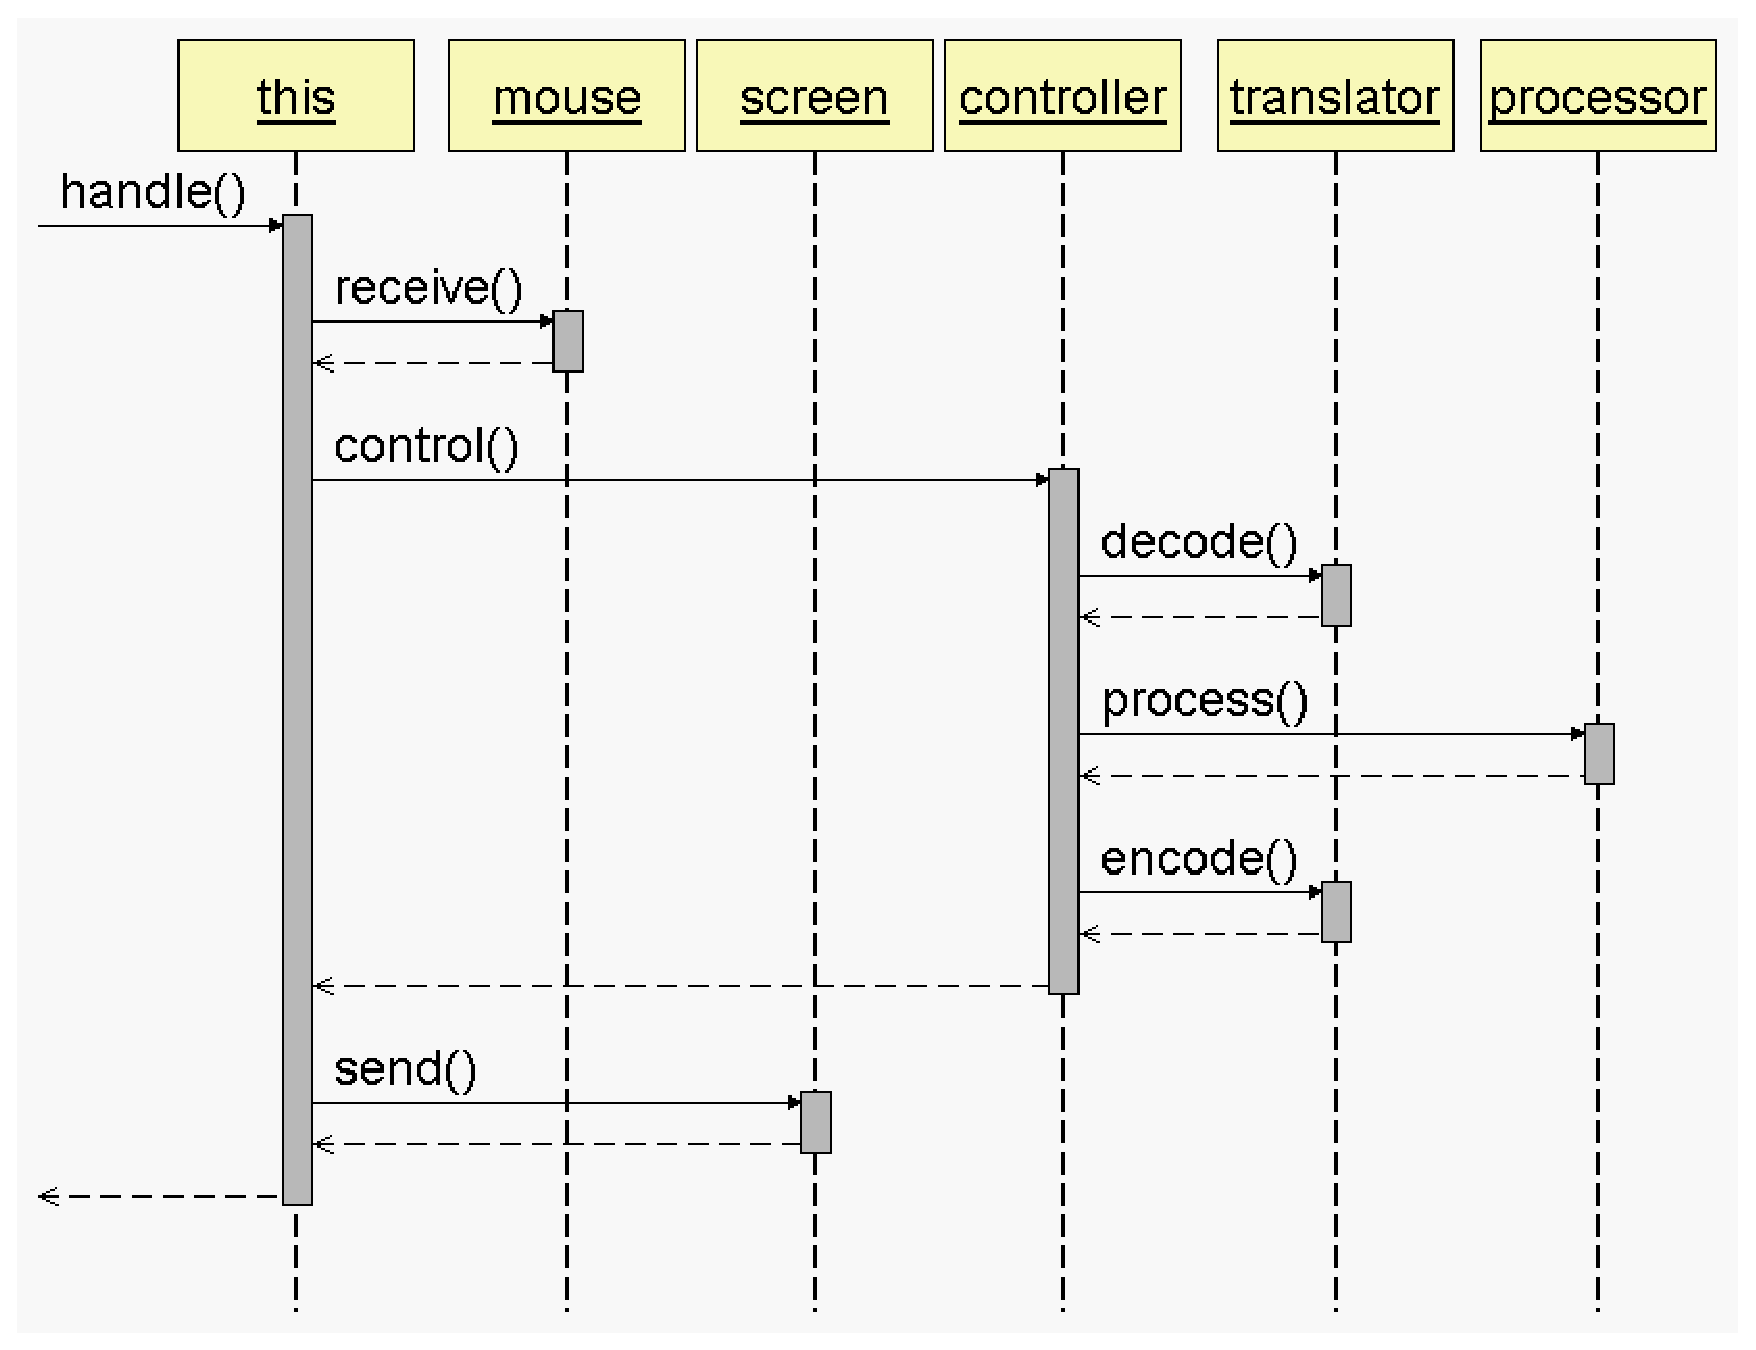
\includegraphics[scale=0.3]{vector/signal_processing.eps}
        \caption{Signal Processing as UML Sequence Diagram}
        \label{signal_processing_figure}
    \end{center}
\end{figure}

The following example demonstrates a typical information (signal) processing
procedure (technical names were used instead of biological ones in figure
\ref{signal_processing_figure}; the terms \emph{Mapper} and \emph{Assembler}
are converted and merged into the term \emph{Translator}):\\
One human \emph{System} wants to send another human \emph{System} a message.
It decides for an acoustical \emph{Signal}, formulates a sentence and talks to
the other human \emph{System} (\emph{handle} method). The other human receives the
\emph{Signal} across its ear organ (\emph{Keyboard}, \emph{Mouse}, \emph{Network}).
The \emph{Signal} is then forwarded to the receiver's brain (\emph{Controller})
where a special \emph{Region} responsible for acoustics (\emph{Translator})
translates (\emph{decode} method) the data (\emph{DataTransferModel}) contained
in the \emph{Signal} and sorts them into the human's abstract model of the
surrounding real world (\emph{DomainModel} or \emph{KnowledgeModel}, respectively).
Processing of the signal happens in the cerebral cortex of the brain (\emph{Processor}).
If the addressed listener wants to send an answer \emph{Signal}, it may do so by
triggering a muscle reaction. For this to happen, the motoric brain region (\emph{Translator})
needs to translate (\emph{encode} method) abstract model data (\emph{DomainModel})
into a special communication model (\emph{UserInterfaceModel}) for the answer signal.
Finally, the answer signal will be sent as muscle action (data display on \emph{Screen}).


    %
% $RCSfile: system_models.tex,v $
%
% Copyright (c) 2001-2004. Christian Heller. All rights reserved.
%
% No copying, altering, distribution or any other actions concerning this
% document, except after explicit permission by the author!
% At some later point in time, this document is planned to be put under
% the GNU FDL license. For now, _everything_ is _restricted_ by the author.
%
% http://www.cybop.net
% - Cybernetics Oriented Programming -
%
% http://www.resmedicinae.org
% - Information in Medicine -
%
% @author Christian Heller <christian.heller@tuxtax.de>
%

\section{System Models}
\label{system_models_heading}

So far, the paper has elaborated on the statics (section \ref{logical_architecture_heading})
as well as the dynamic side (section \ref{biological_reflections_heading}) of the
proposed \emph{Translator} pattern.
This section will finally show the overall results in a number of architecture
diagrams.

%
% $RCSfile: translator_pattern.tex,v $
%
% Copyright (c) 2001-2004. Christian Heller. All rights reserved.
%
% No copying, altering, distribution or any other actions concerning this
% document, except after explicit permission by the author!
% At some later point in time, this document is planned to be put under
% the GNU FDL license. For now, _everything_ is _restricted_ by the author.
%
% http://www.cybop.net
% - Cybernetics Oriented Programming -
%
% http://www.resmedicinae.org
% - Information in Medicine -
%
% @author Christian Heller <christian.heller@tuxtax.de>
%

\subsection{Translator Pattern}
\label{translator_pattern_heading}

As could be seen in section \ref{biological_reflections_heading}, there is always
a \emph{Translator} that is able to map domain model data to communication model
data (\emph{encode} method) and back (\emph{decode} method). Depending on which
communication medium is used, different translators need to be applied (figure
\ref{translator_classes_figure}).

\begin{figure}[ht]
    \begin{center}
        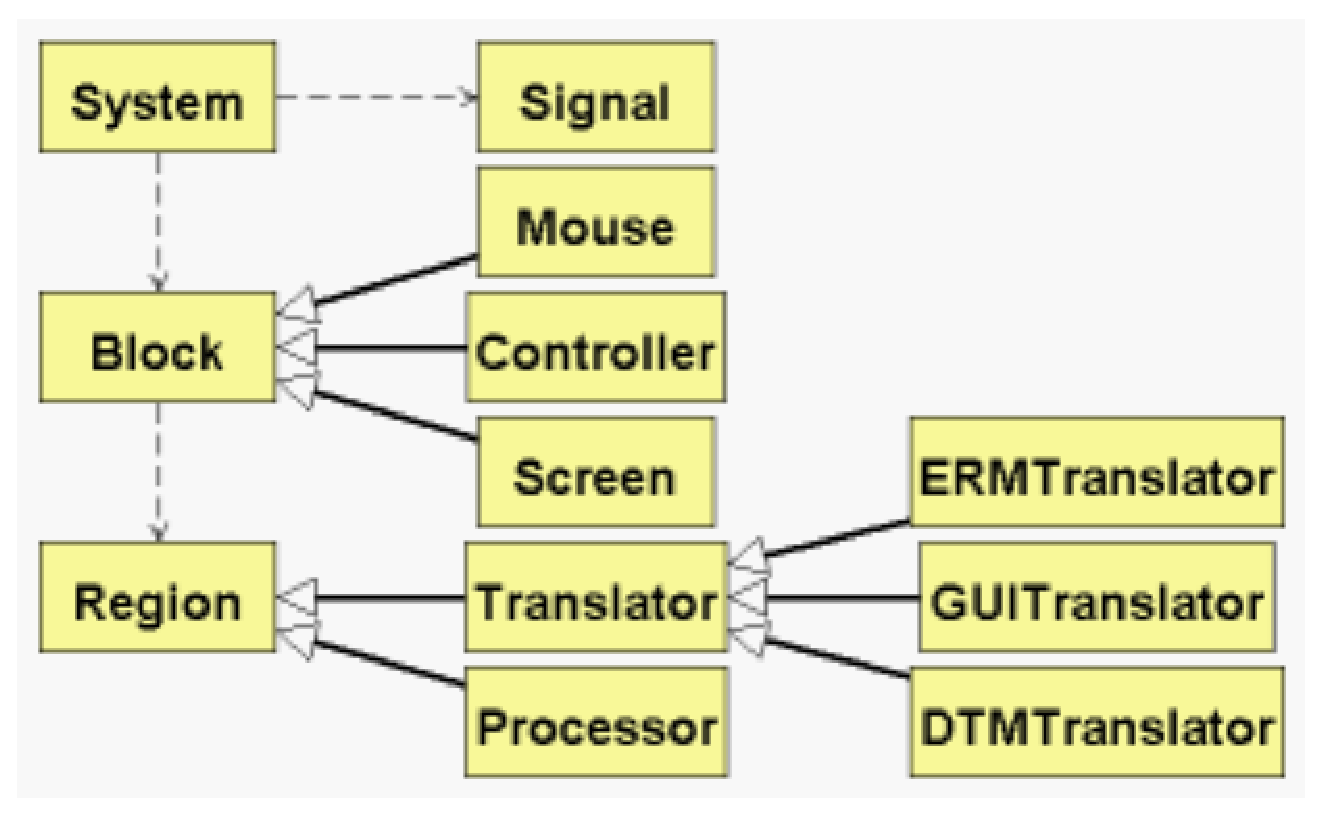
\includegraphics[scale=0.3]{vector/translator_classes.eps}
        \caption{Translator Classes in a UML Class Diagram}
        \label{translator_classes_figure}
    \end{center}
\end{figure}

Every system has exactly one domain model but communication models of arbitrary
type can be added anytime (figure \ref{translator_accessing_models_figure}). Every
translator knows only how to translate between the domain model and a special
communication model. Direct translation between communication models is forbidden
as it would break the flexibility of the whole framework. In other words,
translations always have to be done \emph{via} the domain model.

\begin{figure}[ht]
    \begin{center}
        \includegraphics[scale=0.4]{vector/translator_accessing_models.eps}
        \caption{Translator accessing various Models}
        \label{translator_accessing_models_figure}
    \end{center}
\end{figure}


%
% $RCSfile: ontology_framework.tex,v $
%
% Copyright (c) 2001-2004. Christian Heller. All rights reserved.
%
% No copying, altering, distribution or any other actions concerning this
% document, except after explicit permission by the author!
% At some later point in time, this document is planned to be put under
% the GNU FDL license. For now, _everything_ is _restricted_ by the author.
%
% http://www.cybop.net
% - Cybernetics Oriented Programming -
%
% http://www.resmedicinae.org
% - Information in Medicine -
%
% @author Christian Heller <christian.heller@tuxtax.de>
%

\subsection{Ontology Framework}
\label{ontology_framework_heading}

When placing the translators of figure \ref{translator_classes_figure} into the
greater system architecture context, a \emph{System Ontology} as shown in
figure \ref{system_ontology_figure} may be retrieved. It contains the new
\emph{Translator} as sub class of \emph{Region}, input/ output devices as sub
class of \emph{Block}, \emph{Module} (\emph{Application}) and \emph{User} as sub
class of \emph{System} and further parts which are not the topic of this paper.
For the ease of understanding, the biological counterparts have been added on
the right side of the figure.\\
Specialized translators may be derived as sub class of the one shown in figure
\ref{system_ontology_figure}.

\begin{figure}[ht]
    \begin{center}
        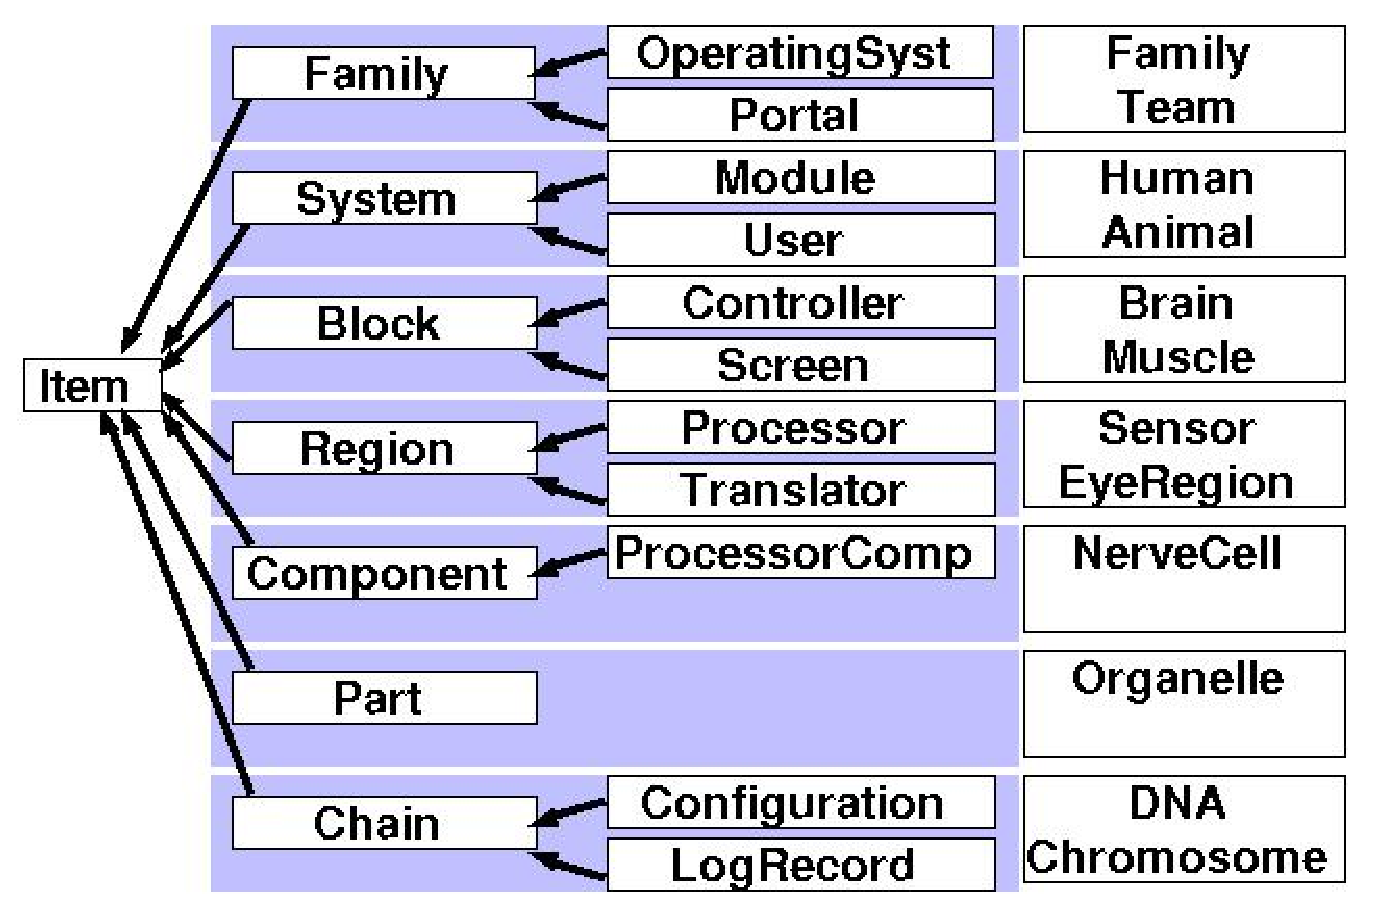
\includegraphics[scale=0.3]{vector/system_ontology.eps}
        \caption{System Ontology}
        \label{system_ontology_figure}
    \end{center}
\end{figure}

To complete the list of important ontology models, figure \ref{basic_ontology_figure}
gives an overview of language-integrated types (commonly called \emph{Primitives}).
And as a matter of fact: All typecasted programming languages already contain an
\emph{Ontology}!
These primitives represent the lowest layer in an ontology or in other words, the
last level of abstraction in software. That is also where \emph{Terminologies}
(that are mostly mentioned in conjunction with ontologies) come in. Basically,
these are sorted collections of terms (strings) but not further elaborated here.

\begin{figure}[ht]
    \begin{center}
        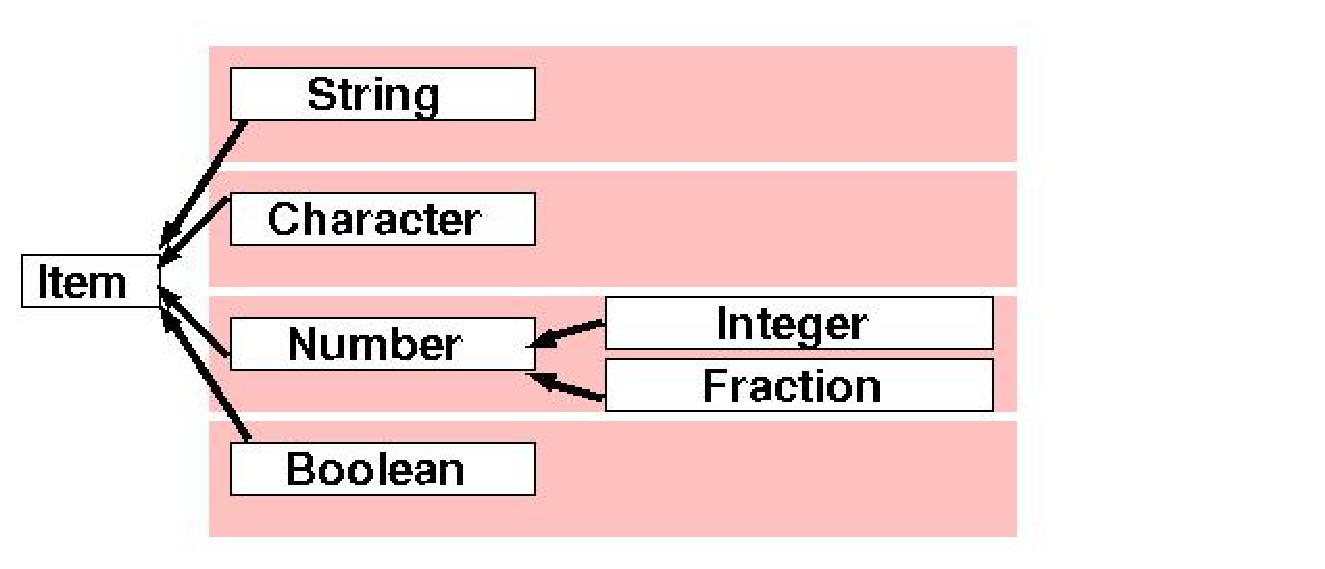
\includegraphics[scale=0.4]{vector/basic_ontology.eps}
        \caption{Basic (Language) Ontology}
        \label{basic_ontology_figure}
    \end{center}
\end{figure}

Putting the three ontologies \emph{Basic}, \emph{Model} and \emph{System} that were
introduced in this paper together, results in the CYBOP architecture of figure
\ref{ontology_framework_figure}. All ontologies base on the \emph{Language Ontology}.
A system built after the \emph{System Ontology} model (in this paper the example
of an \emph{Electronic Health Record} application) may access one ore more
\emph{Model Ontologies} (in the example the health record domain model).
All dependencies are unidirectional.

\begin{figure}[ht]
    \begin{center}
        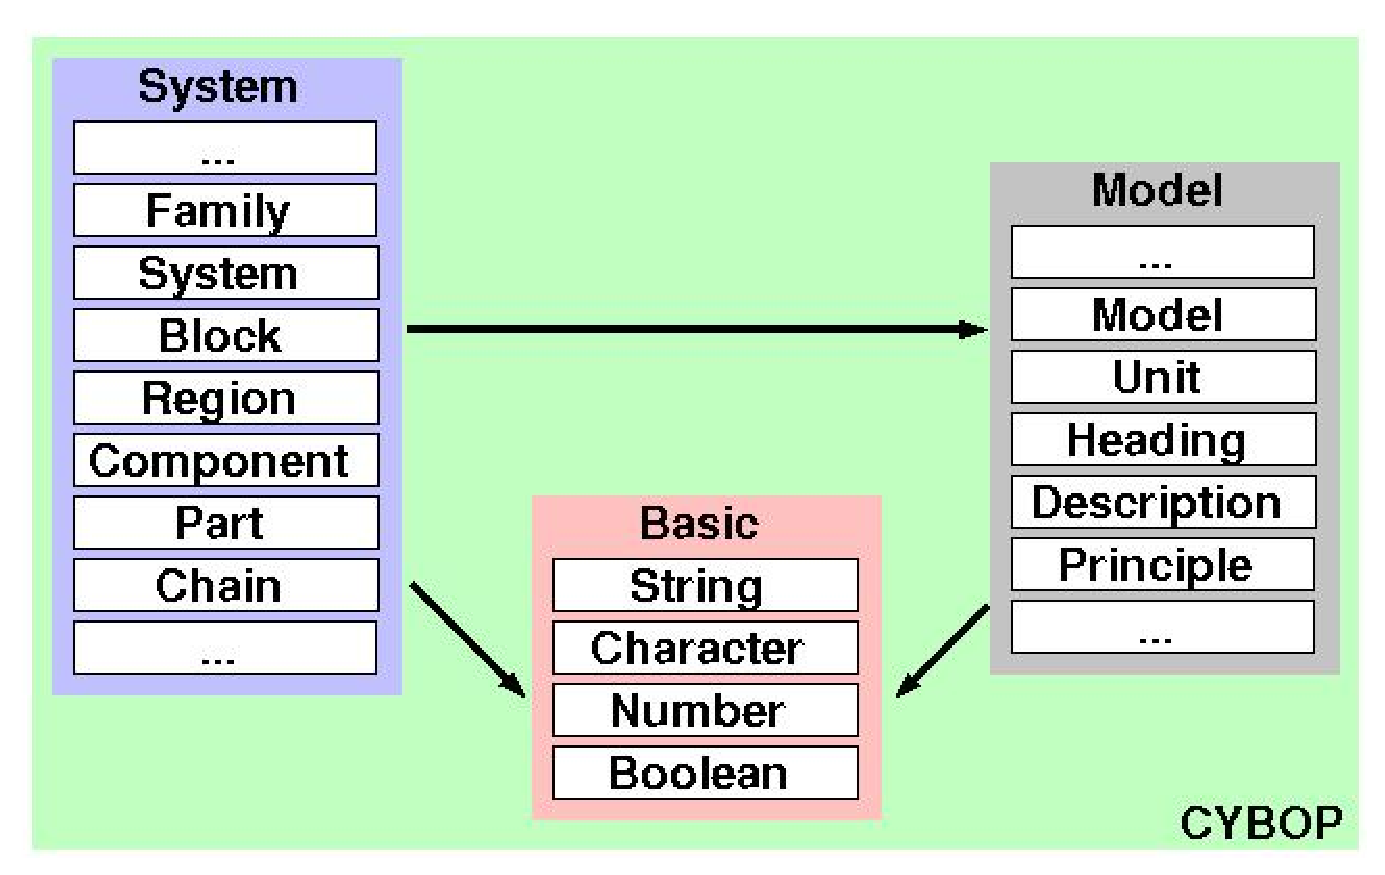
\includegraphics[scale=0.3]{vector/ontology_framework.eps}
        \caption{CYBOP Ontology Framework}
        \label{ontology_framework_figure}
    \end{center}
\end{figure}


%
% $RCSfile: consistency.tex,v $
%
% Copyright (c) 2001-2004. Christian Heller. All rights reserved.
%
% No copying, altering, distribution or any other actions concerning this
% document, except after explicit permission by the author!
% At some later point in time, this document is planned to be put under
% the GNU FDL license. For now, _everything_ is _restricted_ by the author.
%
% http://www.cybop.net
% - Cybernetics Oriented Programming -
%
% http://www.resmedicinae.org
% - Information in Medicine -
%
% @author Christian Heller <christian.heller@tuxtax.de>
%

\subsection{Consistency}
\label{consistency_heading}

The described models are highly flexible and extensible and absolutely transparent
to the user (developer). S/he will not know whether the current communication is
with the local file system, a database or a remote process on another machine.\\
However, this transparency causes a number of problems. Surely, the most common
question is how to ensure consistency, security and minimum redundance?
The following two paragraphs give an answer to the first part of this question
-- consistency and uniqueness of data sets. Maximizing security and minimizing
redundancy have to be analysed in future works.

%
% $RCSfile: object_id.tex,v $
%
% Copyright (c) 2001-2004. Christian Heller. All rights reserved.
%
% No copying, altering, distribution or any other actions concerning this
% document, except after explicit permission by the author!
% At some later point in time, this document is planned to be put under
% the GNU FDL license. For now, _everything_ is _restricted_ by the author.
%
% http://www.cybop.net
% - Cybernetics Oriented Programming -
%
% http://www.resmedicinae.org
% - Information in Medicine -
%
% @author Christian Heller <christian.heller@tuxtax.de>
%

\subsubsection{Object ID (OID)}
\label{object_id_heading}

Most database systems provide an own algorithm to generate primary keys for the
tables. But the applications that use our communication architecture shall also
be able to work if a database server is not reachable, e.g. due to a network
failure. Thats why the keys are generated locally, by each application.
Based on the assumption that every host in a network has a network card, it thereby
has a unique internet address. This number is concatinated with an exact time stamp
(nanoseconds). That is why the OID is unique in the global network and unique in
time.\\
The proposed approach uses the OID as file name for local storage and the same
OID as primary key in the main table of the database. Therewith, both models can
be mapped to each other. Of course, it is necessary to avoid overwriting of new
data in the database. If, for example, a network connection is cut and a little
later, one wants to get data from the local files and write them up in the restored
central database, it has to be made sure that nobody else has modified the data
during the offline-time. That is why there is another technique to ensure this
-- the time stamp.


%
% $RCSfile: time_stamp.tex,v $
%
% Copyright (c) 2001-2004. Christian Heller. All rights reserved.
%
% No copying, altering, distribution or any other actions concerning this
% document, except after explicit permission by the author!
% At some later point in time, this document is planned to be put under
% the GNU FDL license. For now, _everything_ is _restricted_ by the author.
%
% http://www.cybop.net
% - Cybernetics Oriented Programming -
%
% http://www.resmedicinae.org
% - Information in Medicine -
%
% @author Christian Heller <christian.heller@tuxtax.de>
%

\subsubsection{Time Stamp}
\label{time_stamp_heading}

Most database developers will know this technique. Each table has a separate
column for storing the time at which the data were written into this table.
If someone requests information from the database, the time stamp is delivered
as well. After modifying the data, they have to be written back into the database.
At this time, both timestamps (the one in the database table and the one delivered
before) are compared. If there is a difference, the data were modified by another
user. Then, one has to care about the update without overwriting the new data in
the table.






    %
% $RCSfile: physical_architecture.tex,v $
%
% Copyright (c) 2001-2004. Christian Heller. All rights reserved.
%
% No copying, altering, distribution or any other actions concerning this
% document, except after explicit permission by the author!
% At some later point in time, this document is planned to be put under
% the GNU FDL license. For now, _everything_ is _restricted_ by the author.
%
% http://www.cybop.net
% - Cybernetics Oriented Programming -
%
% http://www.resmedicinae.org
% - Information in Medicine -
%
% @author Christian Heller <christian.heller@tuxtax.de>
%

\section{Physical Architecture}
\label{physical_architecture_heading}

This section wants to give practical proof of the theoretical models described
before. It first introduces the project \emph{Res Medicinae} in whose frame the
software was written. Afterwards, two solutions of a physical architecture,
\emph{Two-Tier} and \emph{Three-Tier} are explained.

%
% $RCSfile: res_medicinae.tex,v $
%
% Copyright (C) 2002-2008. Christian Heller.
%
% Permission is granted to copy, distribute and/or modify this document
% under the terms of the GNU Free Documentation License, Version 1.1 or
% any later version published by the Free Software Foundation; with no
% Invariant Sections, with no Front-Cover Texts and with no Back-Cover
% Texts. A copy of the license is included in the section entitled
% "GNU Free Documentation License".
%
% http://www.cybop.net
% - Cybernetics Oriented Programming -
%
% http://www.resmedicinae.org
% - Information in Medicine -
%
% Version: $Revision: 1.1 $ $Date: 2008-08-19 20:41:08 $ $Author: christian $
% Authors: Christian Heller <christian.heller@tuxtax.de>
%

\chapter{Res Medicinae}
\label{res_medicinae_heading}
\index{Res Medicinae Application Prototype}

\begin{flushright}
    \textsl{
        No Road can ever be too long,\\
        side-by-side with a good Friend.
    }\\
    \textsc{Unknown Author}
\end{flushright}

The first two chapters (\ref{cybernetics_oriented_language_heading} and
\ref{cybernetics_oriented_interpreter_heading}) of part \ref{proof_heading} of
this work defined the CYBOL language and its corresponding interpreter CYBOI.
Since a theory is worth more if it can be proven in practice, this chapter will
describe an effort trying to apply both to create an application system named
\emph{Res Medicinae} \cite{resmedicinae} (Latin for \emph{Matter of Medicine}).

%
% $RCSfile: project.tex,v $
%
% Copyright (C) 2002-2008. Christian Heller.
%
% Permission is granted to copy, distribute and/or modify this document
% under the terms of the GNU Free Documentation License, Version 1.1 or
% any later version published by the Free Software Foundation; with no
% Invariant Sections, with no Front-Cover Texts and with no Back-Cover
% Texts. A copy of the license is included in the section entitled
% "GNU Free Documentation License".
%
% http://www.cybop.net
% - Cybernetics Oriented Programming -
%
% http://www.resmedicinae.org
% - Information in Medicine -
%
% Version: $Revision: 1.1 $ $Date: 2008-08-19 20:41:08 $ $Author: christian $
% Authors: Christian Heller <christian.heller@tuxtax.de>
%

\section{Project}
\label{project_heading}
\index{Res Medicinae Project}
\index{Hospital Information System}
\index{HIS}
\index{Practice Management System}
\index{PMS}
\index{Electronic Health Record}
\index{EHR}

The -- somewhat idealistic -- aim was initially to create the prototype of a
\emph{Hospital Information System} (HIS). Due to the clearly too high-set aims,
this was later revised so that the focus of the prototype became a standard
\emph{Practice Management System} (PMS) with an \emph{Electronic Health Record}
(EHR) as its core. Several technology changes during the progress of this work
and the lack in time required to also revise this aim, so that now the final
prototype consists of just the (rudimentary) address management module of the
planned EHR application. It is written in CYBOL and executable by CYBOI.

The following sections describe the project background of \emph{Res Medicinae}.

\input{free_and_open_source_software}
\input{portals_and_services}
\input{tools}
\input{contributors}

%
% $RCSfile: analysis.tex,v $
%
% Copyright (C) 2002-2008. Christian Heller.
%
% Permission is granted to copy, distribute and/or modify this document
% under the terms of the GNU Free Documentation License, Version 1.1 or
% any later version published by the Free Software Foundation; with no
% Invariant Sections, with no Front-Cover Texts and with no Back-Cover
% Texts. A copy of the license is included in the section entitled
% "GNU Free Documentation License".
%
% http://www.cybop.net
% - Cybernetics Oriented Programming -
%
% http://www.resmedicinae.org
% - Information in Medicine -
%
% Version: $Revision: 1.1 $ $Date: 2008-08-19 20:41:05 $ $Author: christian $
% Authors: Christian Heller <christian.heller@tuxtax.de>
%

\section{Analysis}
\label{analysis_heading}
\index{Res Medicinae Requirements Analysis}
\index{Software Engineering Process}
\index{SEP}
\index{Electronic Health Record}
\index{EHR}

Abiding by the standard \emph{Software Engineering Process} (SEP) (chapter
\ref{software_engineering_process_heading}), a \emph{Requirements Analysis}
stood as first activity for the development of \emph{Res Medicinae}. The
following sections will give a brief overview of some requirements and current
modelling trends, concerning the \emph{Electronic Health Record} (EHR). They do
\emph{not} try to replace more comprehensive works written on the subject.

\input{requirements_document}
\input{ehr_and_co}
\input{episode_based}
\input{evidence_based}
\input{continuity_of_care}
\input{core_model}

\newpage
%
% $RCSfile: standards.tex,v $
%
% Copyright (C) 2002-2008. Christian Heller.
%
% Permission is granted to copy, distribute and/or modify this document
% under the terms of the GNU Free Documentation License, Version 1.1 or
% any later version published by the Free Software Foundation; with no
% Invariant Sections, with no Front-Cover Texts and with no Back-Cover
% Texts. A copy of the license is included in the section entitled
% "GNU Free Documentation License".
%
% http://www.cybop.net
% - Cybernetics Oriented Programming -
%
% http://www.resmedicinae.org
% - Information in Medicine -
%
% Version: $Revision: 1.1 $ $Date: 2008-08-19 20:41:09 $ $Author: christian $
% Authors: Christian Heller <christian.heller@tuxtax.de>
%

\section{Standards}
\label{standards_heading}
\index{Medical Informatics Standards}

In a further thought, current standards of medical informatics had to be
considered for the development of \emph{Res Medicinae} application modules.
There exists a whole plethora of (partly \emph{de facto}) standards -- far too
many to discuss here. The following sections will give a brief overview of only
a few standards which are potentially important for EHR development.

\input{overview}
\input{record_modelling}
\input{messaging_and_communication}
\input{terminology_systems}
\input{further_standards}
\input{standards_development}
\input{implication}

%
% $RCSfile: realisation.tex,v $
%
% Copyright (C) 2002-2008. Christian Heller.
%
% Permission is granted to copy, distribute and/or modify this document
% under the terms of the GNU Free Documentation License, Version 1.1 or
% any later version published by the Free Software Foundation; with no
% Invariant Sections, with no Front-Cover Texts and with no Back-Cover
% Texts. A copy of the license is included in the section entitled
% "GNU Free Documentation License".
%
% http://www.cybop.net
% - Cybernetics Oriented Programming -
%
% http://www.resmedicinae.org
% - Information in Medicine -
%
% Version: $Revision: 1.1 $ $Date: 2008-08-19 20:41:08 $ $Author: christian $
% Authors: Christian Heller <christian.heller@tuxtax.de>
%

\section{Realisation}
\label{realisation_heading}
\index{Res Medicinae Steps of Realisation}

Having analysed the domain of healthcare and having investigated corresponding
standards, actual design solutions that have been tried out in the course of
this work, by implementing them in software source code, can be described in
the following sections.

\input{student_works}
\input{first_trial}
\input{knowledge_separation}
\input{reimplementation}
\input{module_modelling}


\input{two_tier_architecture}
%
% $RCSfile: three_tier_architecture.tex,v $
%
% Copyright (c) 2001-2004. Christian Heller. All rights reserved.
%
% No copying, altering, distribution or any other actions concerning this
% document, except after explicit permission by the author!
% At some later point in time, this document is planned to be put under
% the GNU FDL license. For now, _everything_ is _restricted_ by the author.
%
% http://www.cybop.net
% - Cybernetics Oriented Programming -
%
% http://www.resmedicinae.org
% - Information in Medicine -
%
% @author Christian Heller <christian.heller@tuxtax.de>
%

\subsection{Three Tier Architecture}
\label{three_tier_architecture_heading}

To provide a more comfortable structure than the typical \emph{Two-Tier}
architecture as shown in section \ref{two_tier_architecture_heading}, there is
the necessity of a \emph{Three-} or \emph{Multi-Tier} Architecture.
If, for example, the location of the database server was changed then, in a
\emph{Two-Tier} architecture, all clients would have to be updated.
Figure \ref{three_tier_architecture_figure} makes a proposition to solve
this problem.

\begin{figure}[ht]
    \begin{center}
       \includegraphics[scale=0.45]{vector/three_tier_architecture.eps}
       \caption{Three Tier Architecture}
       \label{three_tier_architecture_figure}
    \end{center}
\end{figure}




    %
% $RCSfile: summary.tex,v $
%
% Copyright (c) 2001-2004. Christian Heller. All rights reserved.
%
% Permission is granted to copy, distribute and/or modify this document
% under the terms of the GNU Free Documentation License, Version 1.1
% or any later version published by the Free Software Foundation;
% with no Invariant Sections, with no Front-Cover Texts and with no Back-Cover
% Texts. A copy of the license is included in the section entitled
% "GNU Free Documentation License".
%
% http://www.cybop.net
% - Cybernetics Oriented Programming -
%
% http://www.resmedicinae.org
% - Information in Medicine -
%
% @author Christian Heller <christian.heller@tuxtax.de>
% @author Jens Bohl <info@jens-bohl.de>
%

\section{Summary}
\label{summary_heading}

Software design patterns are essential elements of frameworks. They can be
combined to comprise their advantages and to realize hierarchical structures.
These structures can be created and destroyed in the lifecycle of components.
In that lifecycle, object relations become more transparent and are easier to
control and to maintain.\\
Ontologies can help to model particular domains and to layer software. Every level
of these ontologies has a particular supertype, whereby these types depend on each
other by inheritance. This concept supports the modelling and logical separation
of software into hierarchical architectures. The granularity of the ontology
(number of ontological levels) can be adapted to particular requests.\\
By applying the new concepts introduced in this document, the quality of software
can be greatly increased. The time for building systems can be reduced to a minimum.
The clear architecture avoids common confusion as the systems grow.


    %
% $RCSfile: acknowledgements.tex,v $
%
% Copyright (c) 2001-2004. Christian Heller. All rights reserved.
%
% No copying, altering, distribution or any other actions concerning this
% document, except after explicit permission by the author!
% At some later point in time, this document is planned to be put under
% the GNU FDL license. For now, _everything_ is _restricted_ by the author.
%
% http://www.cybop.net
% - Cybernetics Oriented Programming -
%
% http://www.resmedicinae.org
% - Information in Medicine -
%
% @author Christian Heller <christian.heller@tuxtax.de>
%

\section{Acknowledgements}
\label{acknowledgements_heading}

Our special thanks go to all Enthusiasts of the Open Source Community who have
provided us with a great amount of knowledge through a comprising code base to
build on. We'd also like to acknowledge the contributors of \emph{Res Medicinae},
especially all medical doctors who supported us with their analysis work
\cite{resmedicinae2001} and specialised knowledge in our project mailing lists.
Further on, great thanks goes to the Urban and Fischer publishing company, for
providing anatomical images from their \emph{Sobotta -- Atlas der Anatomie}.


    \label{references_heading}
    \bibliographystyle{geralpha}
    \bibliography{references}
\end{document}

